\chapter{METHODOLOGY}
%\section{Introduction}
%This chapter covers the development of the MOAPTEx family of distributions. It includes deriving its properties, evaluation techniques using Monte Carlo simulations and approaches for assessing model performance and goodness of fit.

\section{Modeling and Analysis of Quadrotor
 Flight Dynamics}
 
\subsection{Preliminary Notions of Quadrotor UAV}

Quadrotor is a type of UAV which holds electronic board at the middle, and a pair of propellers on the rotor of Brushless DC (BLDC) motors\cite{mohidem2022application} at four extremities. There are two possible configurations in Quad design such as ``Plus (+)'' configuration in which a single rotor leads the Quad, and ``Cross (X)'' configuration where two rotors lead the Quad. However, the most popular one is X-configuration since it is more stable and doesn’t have camera obstruction. To command thrust, roll, pitch, and yaw independently, propellers at the opposite ends of the same arm rotate in the same direction in the way that pair of propellers on one arm rotate clockwise (CW) while the other pair rotate in counter clockwise (CCW) direction\cite{akhil2012simulation}.

%%%%%%%%%%%%%%%%%%%%%%%%%%%%5
%The figures in Figure \ref{fig:Types of Quad configuration hover and pitch} and \ref{fig:Types of Quad configuration roll and yaw}, illustrate quadcopter flight maneuvers through differential motor speed control, where red, orange, and blue represent high, medium, and low propeller speeds respectively. 

%\textbf{Hover:} All four motors ($\Omega_1, \Omega_2, \Omega_3, \Omega_4$) operate at equal high speeds (red), generating balanced thrust to maintain stationary flight in both Plus and X configurations.

%\textbf{Pitch Up:} Front motors ($\Omega_1, \Omega_2$) increase to high speed (red) while rear motors ($\Omega_3, \Omega_4$) reduce to low speed (blue), creating forward tilting moment about the lateral axis.

%\textbf{Right Roll:} Left side motors increase to high speed (red) while right side motors decrease to low speed (blue), generating rightward rolling moment about the longitudinal axis.

%\textbf{Clockwise Yaw:} Diagonal motor pairs operate at different speeds clockwise rotating motors increase while counter clockwise motors decrease producing net yaw torque without altitude change, enabling rotation about the vertical axis.
%%%%%%%%%%%%%%%%%%%%%%%%%%

Depending on the angular speed of each propeller, it is possible to determine the direction of Quadrotor maneuvering as shown in Figure \ref{fig:quad_config} where the color of arrow inside the propellers are proportional to the magnitude of angular speed of the propellers meaning that red,orange and green represents High,Medium and Low speed respectively.

%\begin{figure}[h!]
    %\centering
    %\includegraphics[width=0.5\linewidth]{Figures/Types of Quad configuration, and its relative motion w.r.t propeller speed.PNG}
   % \caption{Types of Quad configuration, and its relative motion w.r.t propeller speed\cite{wallace2016dynamics}}
    %\label{fig:Types of Quad configuration}
%\end{figure}

%\begin{figure}[h!]
   % \centering
    %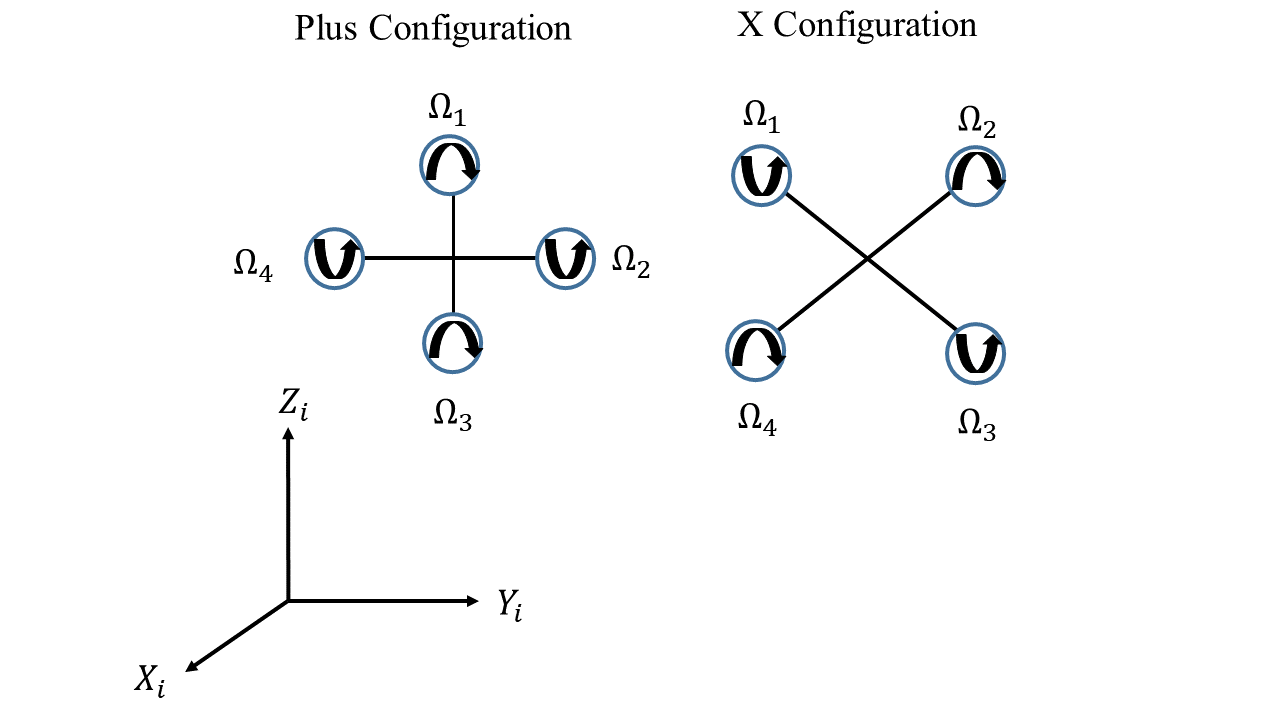
\includegraphics[width=1.0\linewidth]{figures/quad configuration.png}
    % Caption that goes to List of Figures (no citation here)
   % \caption{Types of Quad configuration, and its relative motion w.r.t propeller speed}
    % Extra caption shown only under the figure, with citation
    %\caption*{Source: \cite{wallace2016dynamics}}
   % \label{fig:Types of Quad configuration}
%\end{figure}

%\begin{figure}[h!]
   % \centering
   % \begin{minipage}{0.48\linewidth}
      %  \centering
       % 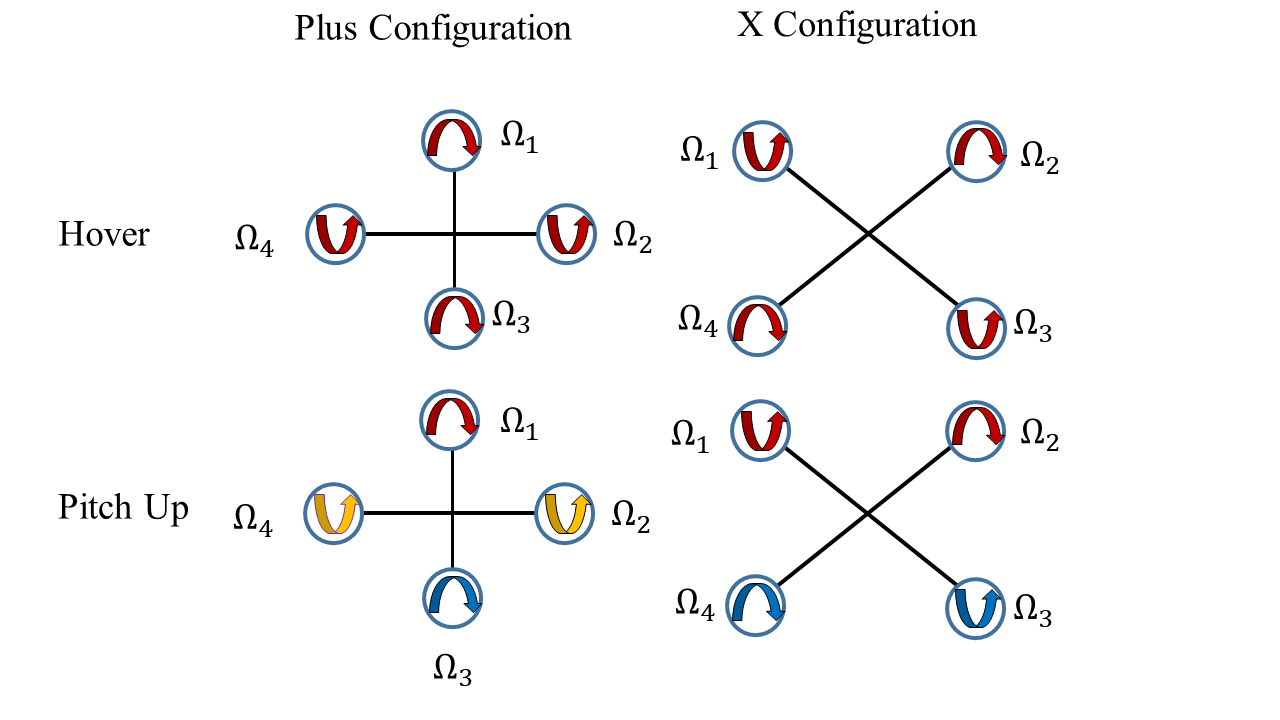
\includegraphics[width=\linewidth]{figures/quad configuration best 1.png}
       % \caption{Types of Quad configuration,  Hover and Pitch up motion with respect propeller speed}
       % \label{fig:Types of Quad configuration hover and pitch}
   % \end{minipage}
   % \hfill
   % \begin{minipage}{0.48\linewidth}
      %  \centering
       % 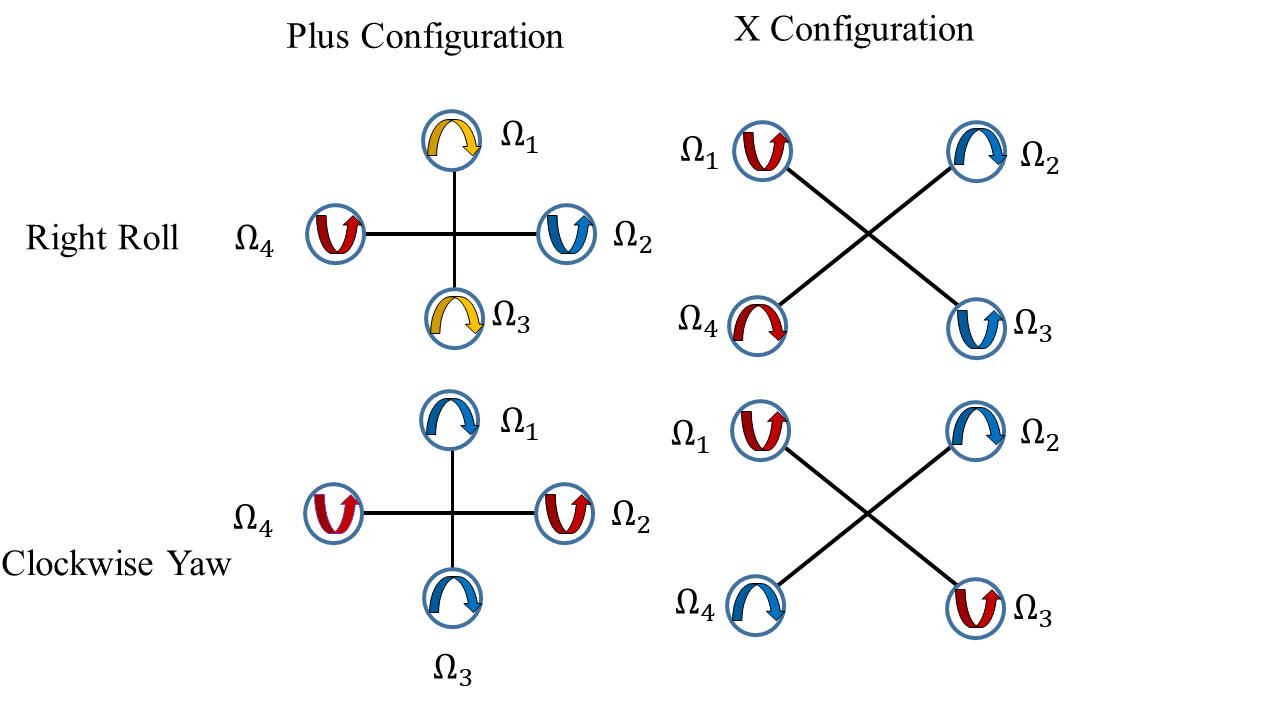
\includegraphics[width=\linewidth]{figures/quad configuration best 2nd.png}
       % \caption{Types of Quad configuration, Roll and Yaw motion with respect propeller speed}
       % \label{fig:Types of Quad configuration roll and yaw}
  %  \end{minipage}
 %\caption{Experimental quadcopter platform and test setup}
    %\label{fig:quadcopter_setup}

    
\end{figure}

\begin{figure}[h!]
    \centering
    \begin{subfigure}{0.48\linewidth}
        \centering
        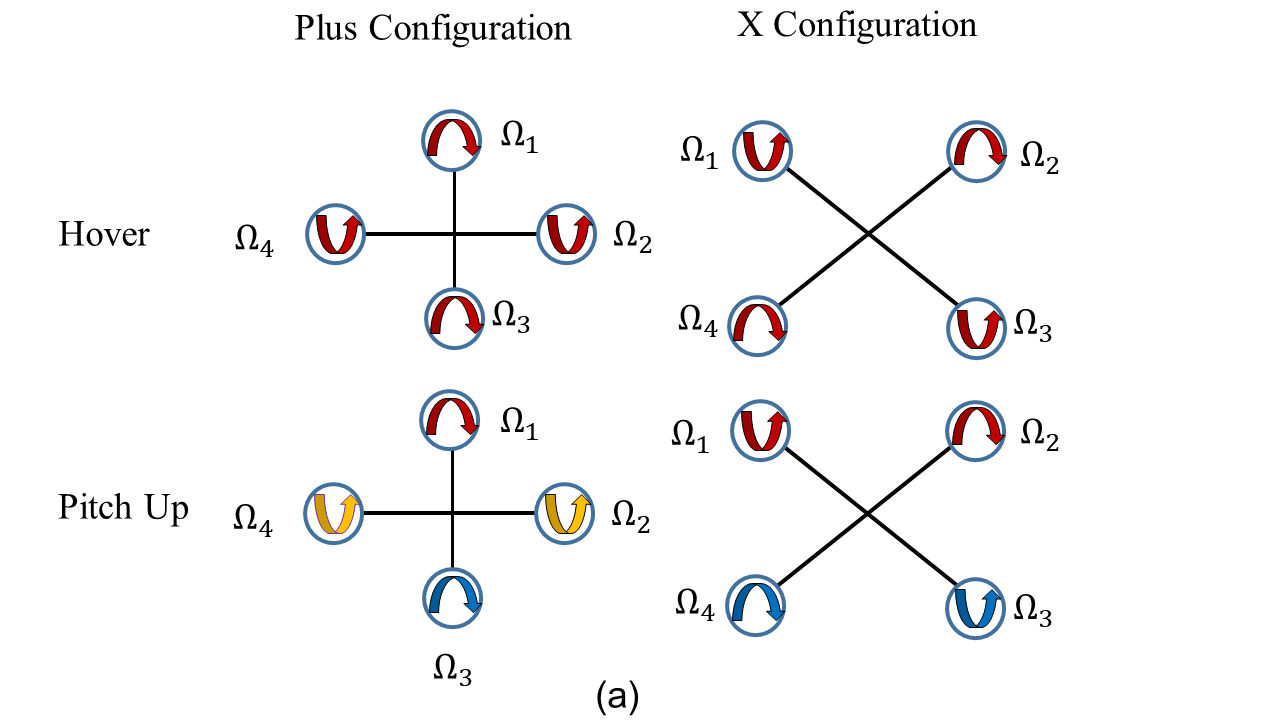
\includegraphics[width=\linewidth]{figures/quad configuration hover and pitch.png}
        \phantomcaption
        \label{fig:quad_a}
    \end{subfigure}
    \hfill
    \begin{subfigure}{0.48\linewidth}
        \centering
        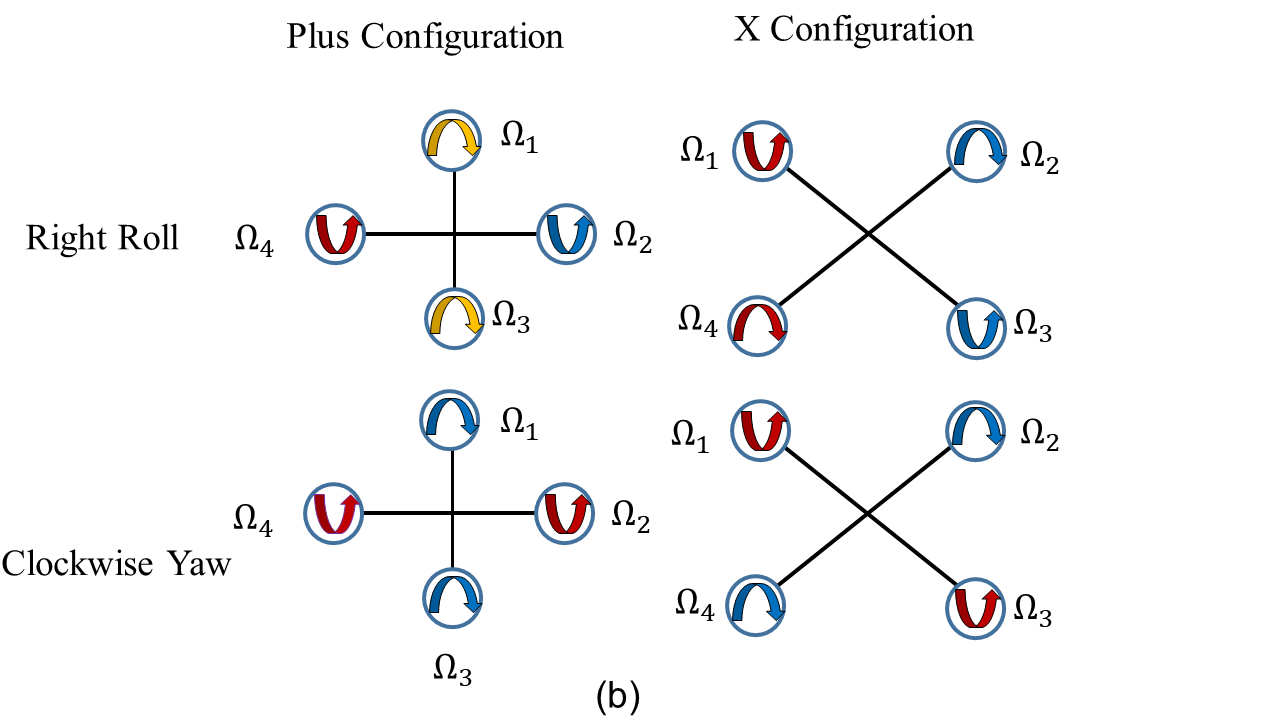
\includegraphics[width=\linewidth]{figures/quad configuration roll and yaw.png}
        \phantomcaption
        \label{fig:quad_b}
    \end{subfigure}

    \caption{Types of quadcopter configurations showing motion generation through propeller speed variation: (a) hover and pitch motion, (b) roll and yaw motion.}
    \label{fig:quad_config}
\end{figure}




Flight mode of Quadrotor can be controlled to desired pose in the space by changing the direction and velocity of each propellers\cite{alemaw2019precision}. The thrust forces caused by propellers rotation are responsible for ascending or descending flight. As shown in Figure  \ref{fig:quad_config} (b), applying speed difference between side propellers result in roll rotation coupled with y-axis translation. Similarly the pitch rotation coupled with translation motion along x-axis is caused due to the speed difference between front and rear propellers as shown in Figure  \ref{fig:quad_config} (a). The yaw rotation is caused due to unbalanced rotation speed of the four propellers. Unlike the roll and pitch rotation, yaw rotation is the result of reactive torques shown below which can be found also in Figure.\ref{fig:Quadrotor free body diagram} 

\[
\tau_i, \; i = 1,2,3,4 \text{ represents the individual torque of each rotor,}
\]
\[
\Omega_i, \; i = 1,2,3,4 \text{ represents the angular velocity of each rotor.}
\]
Increasing CCW rotated propellers speed result in yaw CW vehicle rotation.
In order to design mathematical model of Quadrotor, the coordinate frame of Quadrotor has to be defined first. There are two coordinate frames, as shown in Figure~\ref{fig:Quadrotor free body diagram}, that the Quadrotor will operate in: inertial or fixed frame $(x_i, y_i, z_i)$ and body or mobile frame $(x_b, y_b, z_b)$\cite{lv2014sliding}. Inertial Frame (IF) is where the Newton laws are valid and defined with respect to the ground with positive z axis pointing in the opposite direction of gravity, whereas Body Frame (BF) is defined with respect to Center of Gravity (CoG) of the Quadrotor with its axes  fixed to the body.
%Here we are going to use the two types of Right Hand Rule: the one in left side used to determine the positive direction of axis of rotation, and the one in right side used to determine direction of angular position where thumb pointing positive direction of axis of rotation and the turned fingers pointing positive direction of angular position.


\begin{figure}[h!]
    \centering
    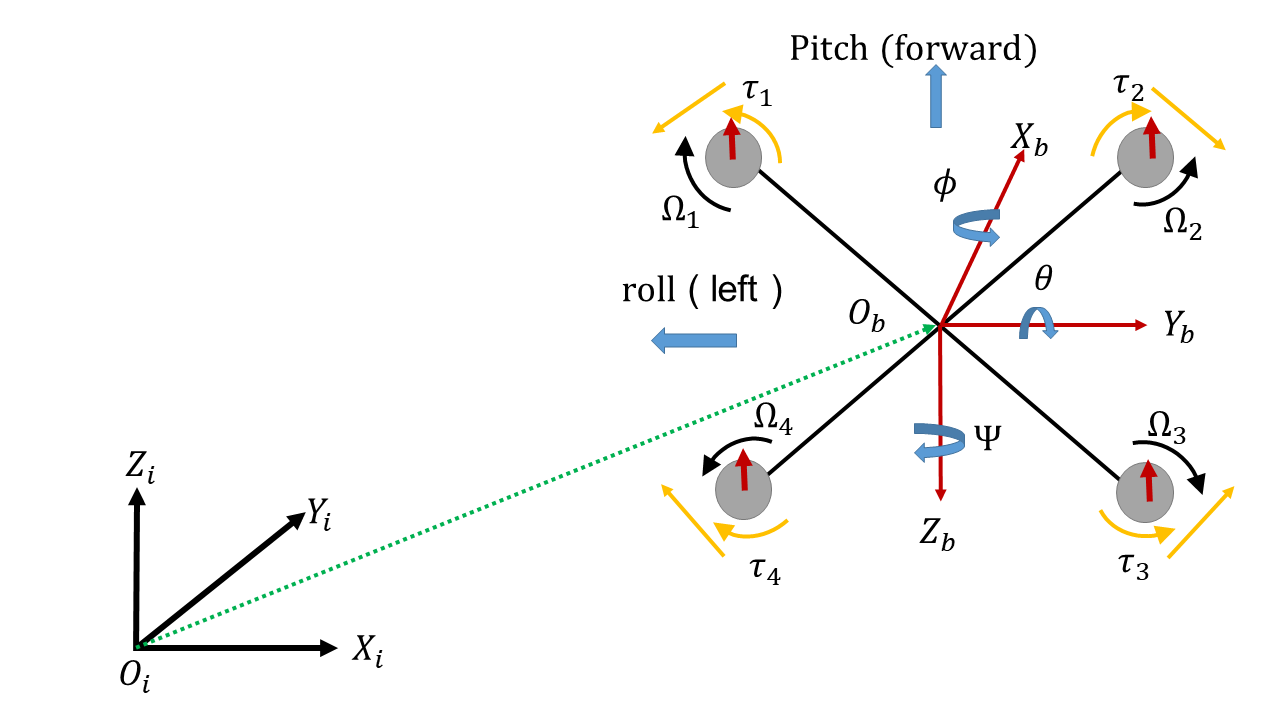
\includegraphics[width=1\linewidth]{figures/Quadcopter FBD.png}
    \caption{Quadrotor free body diagram and its reference frames }
    \label{fig:Quadrotor free body diagram}
\end{figure}





The necessity of diffining those reference frames is because of: actuator inputs $U$ and thrusts $T$, Inertial Measurement Unit (IMU), Accelerometer, Magnetometer  are manipulated and measure quantities with respect to Body Frame (BF). Also  GPS measures position with respect to Inertial Frame and Model development is carried out with respect to IF since Newton laws are valid in IF only.

%\begin{itemize}
    %\item 
    
    %\item Inertial Measurement Unit (IMU), Accelerometer, and Magnetometer measure quantities with respect to BF,
    %\item GPS measures position with respect to IF, and
    %\item Model development is carried out with respect to IF since Newton laws are valid in IF only.
%\end{itemize}

\subsection{Coordinate Frames Transformation}

%Coordinate frames transformation is used to transform quantities between the two reference frames. In this sub-section we are going to see the two most known approaches for coordinate transformation: Euler or classical approach, and Quaternion approach.
Coordinate frames transformation was used to transform quantities between the two reference frames. In this subsection  the  Quaternion approach for coordinate transformation was realized as controller designed  based on this.


%\subsubsubsection{\textbf{Euler or Classical Approach}}

%Euler approach uses three parameters: roll $\phi$, pitch $\theta$, and yaw $\psi$ to describe orientation in 3D space, and it requires three consecutive rotations along roll, pitch and yaw, to transform BF quantities into IF quantities. Since GPS measures position w.r.t IF, single axis rotational matrix can be constructed by projecting IF coordinates into BF coordinates. Projection matrix in terms of dot products of the basis vectors of the two coordinate frames is given as\textsuperscript{[24]}:

%\begin{equation}
%R^b_e =
%\begin{bmatrix}
%X_e \cdot X_b & Y_e \cdot X_b & Z_e \cdot X_b \\
%X_e \cdot Y_b & Y_e \cdot Y_b & Z_e \cdot Y_b \\
%X_e \cdot Z_b & Y_e \cdot Z_b & Z_e \cdot Z_b
%\end{bmatrix}
%\label{eq:rotation_matrix}
%\tag{3.1}
%\end{equation}



%\textit{Euler rotation theorem} states that orientation of 3D coordinate frame w.r.t another can be described by successive rotation about three axes in the way that no two successive rotations are about the same axes. Therefore; Yaw-Roll-Pitch (zyx) sequence rotation matrix, which is the most commonly used conventions from the 12 different possible rotation sequences: xyz, xzy, yxz, yzx, zyx, zxy, xyx, xzx, yyy, yzy, zyz, and zyz\cite{waldron2007handbook}, is taken to project IF quantities into Quadrotor BF quantities as shown in Figure\ref{fig:cordinate frame transformation}.
% \begin{figure}[h!]
%     \centering
%     \includegraphics[width=0.5\linewidth]{Figures/cordinate frame transformation.PNG}
%     \caption{\textit{Coordinate transformation from IF to the BF by using Euler angles} $(\phi, \theta, \psi)$}
%     \label{fig:cordinate frame transformation}
% \end{figure}

 %By using equation (3.1) we can get rotation matrix along z-axis $R_z(\psi)$ as

% \begin{equation}
% R_z(\psi) =
% \begin{bmatrix}
% c_\psi & -s_\psi & 0 \\
% s_\psi &  c_\psi & 0 \\
% 0      &  0      & 1
% \end{bmatrix}
% \tag{3.2}
% \end{equation}

% , along y-axis $R_y(\theta)$ as

% \begin{equation}
% R_y(\theta) =
% \begin{bmatrix}
% c_\theta & 0 & s_\theta \\
% 0        & 1 & 0 \\
% -s_\theta& 0 & c_\theta
% \end{bmatrix}
% \tag{3.3}
% \end{equation}

% , and along x-axis $R_x(\phi)$ as

% \begin{equation}
% R_x(\phi) =
% \begin{bmatrix}
% 1 & 0      & 0 \\
% 0 & c_\phi & -s_\phi \\
% 0 & s_\phi &  c_\phi
% \end{bmatrix}
% \tag{3.4}
% \end{equation}

% Where: $c_\theta = \cos\theta$, $s_\theta = \sin\theta$, and $T_\theta = \tan\theta$

%\textit{\textbf{3D Rotation matrix}} $R^b_e$, which transform IF translational position quantities into the BF coordinates, can be obtained by cascading the single axis rotation matrix that described in equation (3.2--3.4) with matrix multiplication as follows:


% \begin{equation}
% R^b_e = R_z(\psi) \cdot R_y(\theta) \cdot R_x(\phi)
% \tag{3.5a}
% \end{equation}

% \[
% R^b_e =
% \begin{bmatrix}
% c_\psi & -s_\psi & 0 \\
% s_\psi &  c_\psi & 0 \\
% 0      &  0      & 1
% \end{bmatrix}
% \begin{bmatrix}
% c_\theta & 0 & s_\theta \\
% 0        & 1 & 0 \\
% -s_\theta& 0 & c_\theta
% \end{bmatrix}
% \begin{bmatrix}
% 1 & 0      & 0 \\
% 0 & c_\phi & -s_\phi \\
% 0 & s_\phi &  c_\phi
% \end{bmatrix}
% \]

% \[
% \begin{equation}
% R^b_e =
% \begin{bmatrix}
% X_e \cdot X_b & Y_e \cdot X_b & Z_e \cdot X_b \\
% X_e \cdot Y_b & Y_e \cdot Y_b & Z_e \cdot Y_b \\
% X_e \cdot Z_b & Y_e \cdot Z_b & Z_e \cdot Z_b
% \end{bmatrix}
% \label{eq:rotation_matrix}
% \tag{3.1}
% \end{equation}
% \]

% Since determinant of individual rotation matrices is one, the cascade of 3D
% rotation matrices R^b_e also has determinant one, i.e., it is orthogonal.
% Therefore, (R^b_e)^T R^b_e = I, and we have (R^b_e)^T = (R^b_e)^{-1} = R^e_b.
% Thus, the 3D rotation matrix that projects body-frame (BF) quantities to the
% inertial frame (IF), R^e_b, is expressed as:
% \begin{equation}
% R^e_b =
% \begin{bmatrix}
%  c_\psi c_\theta & c_\psi s_\theta s_\phi - s_\psi c_\phi & c_\psi s_\theta c_\phi + s_\psi s_\phi \\
%  s_\psi c_\theta & s_\psi s_\theta s_\phi + c_\psi c_\phi & s_\psi s_\theta c_\phi - c_\psi s_\phi \\
% - s_\theta       & c_\theta s_\phi                        & c_\theta c_\phi
% \end{bmatrix}
% \tag{3.5}
% \end{equation}



% \textit{Transformation matrixes for angular velocities} relate Euler angle rates between IF: $[\dot{\phi}, \dot{\theta}, \dot{\psi}]^T$ and BF: $[p, q, r]^T$. To project BF rates into IF, we first rotate BF around x-axis by roll angle $\phi$, which is then followed by rotating around y-axis by pitch angle $\theta$ and finally around z-axis by yaw angle $\psi$, and these steps are expressed in Figure \ref{fig:Rotational sequence} as

%\begin{figure}[h!]
    %\centering
    %\includegraphics[width=0.5\linewidth]{Figures/Rotate transformation.PNG}
    %\caption{Rotation sequence from roll $\rightarrow$ pitch $\rightarrow$ yaw\cite{en14051232}}
    %\label{fig:Rotational sequence}
%\end{figure}

% \begin{figure}[h!]
%     \centering
%     \includegraphics[width=0.5\linewidth]{Figures/Rotate transformation.PNG}
%
%     % Caption that appears in List of Figures (NO citation here)
%     \caption{Rotation sequence from roll $\rightarrow$ pitch $\rightarrow$ yaw}
%
%     % Caption that appears ONLY under the figure (WITH citation)
%     \caption*{Source: \cite{en14051232}}
%
%     \label{fig:Rotational sequence}
% \end{figure}




% The projections of angular rates which are expressed in the vector of Euler rates in the BF into IF can be done as follows. First, we start from backwards with the last rotation $\dot{\phi}$, this is about x-axis which has the same unit vector with $p$, so no frame transformation is required i.e., trivially $\dot{\phi} = p$. Then, lets look at $\dot{\theta}$ this rotation is about y-axis which lags behind BF axis by a roll rotation, so to bring it to BF axis we need to pre-multiply by $R_x(\phi)$. Finally, $\dot{\psi}$ is about z-axis which lags behind by two rotations, so it’s pre-multiplied by $R_z(\phi)R_y(\theta)$. In the case of BF has different origin than the IF, BF rates are calculated from IF by using the following equation\cite{en14051232}:

% \begin{equation}
% \vec{X} = \vec{X}_o + R^T \vec{X}_b
% \tag{3.6a}
% \end{equation}

% Where: $\vec{X}_o$ is the location of moving origin that expressed in IF coordinates. Since IMU measure quantities w.r.t BF whereas GPS measure Euler parameters w.r.t IF, we project first, IF into BF in terms of Euler parameters. Then by inverting coefficient matrix, transformation matrix that relate BF rates with IF is obtained. To do that we maneuver from BF to IF by using inverse of a single axis rotation matrix in equation (3.2--3.4). Since rotation matrixes are orthogonal, their inverse is equal to transpose of corresponding matrix.  
%
%
%
%\[
%\begin{bmatrix}
%p \\ q \\ r
%\end{bmatrix}
%=
%\begin{bmatrix}
%\dot{\phi} \\ 0 \\ 0
%\end{bmatrix}
%+ R_x^T(\phi)
%\begin{bmatrix}
%0 \\ \dot{\theta} \\ 0
%\end{bmatrix}
%+ R_x^T(\phi) R_y^T(\theta)
%\begin{bmatrix}
%0 \\ 0 \\ \dot{\psi}
%\end{bmatrix}
%\]
%Expanding:
%
% First term
%
% \[
% =
% \begin{bmatrix}
% 1 & 0 & 0 \\
% 0 & c_\phi & s_\phi \\
% 0 & -s_\phi & c_\phi
% \end{bmatrix}
% \begin{bmatrix}
% 0 \\ \dot{\theta} \\ 0
% \end{bmatrix}
% +
% %
% % Second term
% %
% \begin{bmatrix}
% 1 & 0 & 0 \\
% 0 & c_\phi & s_\phi \\
% 0 & -s_\phi & c_\phi
% \end{bmatrix}
% \begin{bmatrix}
% c_\theta & 0 & s_\theta \\
% 0 & 1 & 0 \\
% -s_\theta & 0 & c_\theta
% \end{bmatrix}
% \begin{bmatrix}
% 0 \\ 0 \\ \dot{\psi}
% \end{bmatrix}
% + 
% %
% % Third term
% %
% \begin{bmatrix}
% \dot{\phi} \\ 0 \\ 0
% \end{bmatrix}
% \]

% Simplifying:
%
% \[
% =
% \begin{bmatrix}
% \dot{\phi} \\ c_\phi \dot{\theta} \\ -s_\phi \dot{\theta}
% \end{bmatrix}
% +
% \begin{bmatrix}
% 0 \\ s_\phi s_\theta \dot{\psi} + c_\phi \dot{\psi} \\ c_\phi s_\theta \dot{\psi} - s_\phi \dot{\psi}
% \end{bmatrix}
% \]
%
% Thus,
%
% \begin{equation}
% \begin{bmatrix}
% p \\ q \\ r
% \end{bmatrix}
% =
% \begin{bmatrix}
% 1 & 0 & -s_\theta \\
% 0 & c_\phi & s_\phi c_\theta \\
% 0 & -s_\phi & c_\phi c_\theta
% \end{bmatrix}
% \begin{bmatrix}
% \dot{\phi} \\ \dot{\theta} \\ \dot{\psi}
% \end{bmatrix}
% \tag{3.6b}
% \end{equation}

% However, to drive Quadrotor model we need velocity on IF. So, by inverting the above coefficient matrix, rate transformation matrixes that project BF rates into IF becomes
%
% \begin{equation}
% \begin{bmatrix}
% \dot{\phi} \\
% \dot{\theta} \\
% \dot{\psi}
% \end{bmatrix}
% =
% \begin{bmatrix}
% 1 & s_\phi T_\theta & c_\phi T_\theta \\
% 0 & c_\phi          & -s_\phi \\
% 0 & \tfrac{s_\phi}{c_\theta} & \tfrac{c_\phi}{c_\theta}
% \end{bmatrix}
% \begin{bmatrix}
% p \\ q \\ r
% \end{bmatrix}
% \tag{3.6}
% \end{equation}

\subsection*{\textbf{Quaternion Approach}}

%The idea of Quaternions was first proposed by W.R Hamilton in 1843 \cite{hamilton1866elements} as an extension of the imaginary part of complex numbers. He first realized that complex numbers are a powerful tool to manage rotation in 2-dimensional space, then he supposed that a generalization of the complex numbers would also result in a good tool to manage rotations in 3-dimensional space. This makes quaternion as a hyper complex number with four dimensions, one of which is real while the other three are imaginary, that can be utilized to avoid the nonlinearity, geometric singularity, and computational cost usually associated with the Euler angles\cite{fresk2013full,fresk2013modeling}.


The concept of quaternions was originally introduced by W.R. Hamilton in 1843 \cite{hamilton1866elements} as an extension of complex numbers to higher dimensions. Hamilton recognized that complex numbers provide an elegant framework for representing rotations in two-dimensional space and hypothesized that a generalization to higher dimensions would similarly facilitate rotation operations in three-dimensional space. Consequently, quaternions emerge as hypercomplex numbers comprising four dimensions one real component and three imaginary components which effectively circumvent the nonlinearity, geometric singularities, and computational complexity typically associated with Euler angle representations \cite{fresk2013full,fresk2013modeling}.

%Quaternion contains a scalar part $q_0$, and a three dimensional vector part: $\vec{q} = [q_1, q_2, q_3]$ with orthonormal base $[i, j, k]$  representing $[x, y, z]$ axis that satisfies the following fundamental rules introduced by W.R Hamilton \cite{hamilton1866elements}
%\begin{equation}
%q = (q_0, \vec{q}) = \left( \cos\frac{\theta}{2}, \; \sin\frac{\theta}{2} \, \hat{u} \right)
%\tag{3.1}
%\label{eqn 3.1}
%\end{equation}

%\[
%ij = k = -ji,\quad jk = i = -kj,\quad ki = j = -ik.
%\]

%Hence, \[
%i^2 = j^2 = k^2 = ijk = -1
%\]
%Also there are three common conventions for representing a quaternion:
%\[
%q = q_0 + q_1 \hat{i} + q_2 \hat{j} + q_3 \hat{k}
%= [q_0, q_1, q_2, q_3] = (q_0, \vec{q})
%\]
%%%%%%%%%%%%%%%%%%%%%%%%%%%%%%%%%%%
A quaternion consists of a scalar part $q_0$ and a three-dimensional vector part $\vec{q} = [q_1, q_2, q_3]$, which can be expressed in the form:
\begin{equation}
q = (q_0, \vec{q}) = \left( \cos\frac{\theta}{2}, \sin\frac{\theta}{2} \, \hat{u} \right),
\label{eqn:quaternion_form}
\end{equation}
where $\theta$ represents the rotation angle and $\hat{u}$ is the unit vector along the rotation axis.The vector part is defined with respect to an orthonormal basis $[\hat{i}, \hat{j}, \hat{k}]$ representing the $[x, y, z]$ coordinate axes, respectively. These basis elements satisfy the fundamental multiplication rules introduced by W.R. Hamilton \cite{hamilton1866elements}:
\begin{equation}
ij = k = -ji, \quad jk = i = -kj, \quad ki = j = -ik.
\label{eqn:hamilton_rules}
\end{equation}

From these rules, it follows that:
\begin{equation}
i^2 = j^2 = k^2 = ijk = -1.
\label{eqn:quaternion_squares}
\end{equation}

There are three equivalent conventions commonly used for representing a quaternion:
\begin{equation}
q = q_0 + q_1 \hat{i} + q_2 \hat{j} + q_3 \hat{k} = [q_0, q_1, q_2, q_3] = (q_0, \vec{q}).
\label{eqn:quaternion_representations}
\end{equation}


%%%%%%%%%%%%%%%%%%%%%%%%%%%%%

%In order to represent a valid 3D orientation or to compute valid vector rotations, the quaternion must be normalized. The normalized quaternion is ideally suitable for representing orientation of an object in 3D space and transforming orientation of coordinates between any two reference frames. Quaternion normalization can be done just like a four dimension vector by dividing each of four components by its Euclidean norm, and it’s mathematically expressed as.

%\[
%q = \frac{q_0 + q_1 i + q_2 j + q_3 k}{\sqrt{q_0^2 + q_1^2 + q_2^2 + q_3^2}},
%\]

%Where this normalized quaternion physically interpreted as an angle in 3D space about which a single rotation defines the final orientation of a frame relative to some initial reference frame i.e., it represent orientation by a single rotation around an axis $\hat{u}$ as shown in figure \ref{fig:Quaternion representation of rotation along rotation axis}. In case of Euler rotation theorem, this requires three consecutive rotations about a single axis along yaw, pitch and roll directions.

%%%%%%%%%%%%%%%%%%%%%
For valid representation of 3D orientations and vector rotations, quaternions must be normalized. Normalized quaternions provide an optimal framework for describing object orientations in three-dimensional space and transforming coordinates between reference frames. Normalization follows the standard procedure for four-dimensional vectors, dividing each component by the quaternion's Euclidean norm:
\begin{equation}
%q_{\text{norm}} = \frac{q_0 + q_1 \hat{i} + q_2 \hat{j} + q_3 \hat{k}}{\sqrt{q_0^2 + q_1^2 + q_2^2 + q_3^2}}.
q = \frac{q_0 + q_1 \hat{i} + q_2 \hat{j} + q_3 \hat{k}}{\sqrt{q_0^2 + q_1^2 + q_2^2 + q_3^2}}.
\label{eqn:quaternion_normalization}
\end{equation}

The normalized quaternion physically represents a single rotation about an axis $\hat{u}$ in 3D space, defining the orientation of a frame relative to a reference frame as shown in Figure~\ref{fig:Quaternion representation of rotation along rotation axis}). This contrasts with Euler's rotation theorem, which requires three consecutive rotations about individual axes (yaw, pitch, and roll).


%%%%%%%%%%%%%%%%




\begin{figure}[h!]
    \centering
    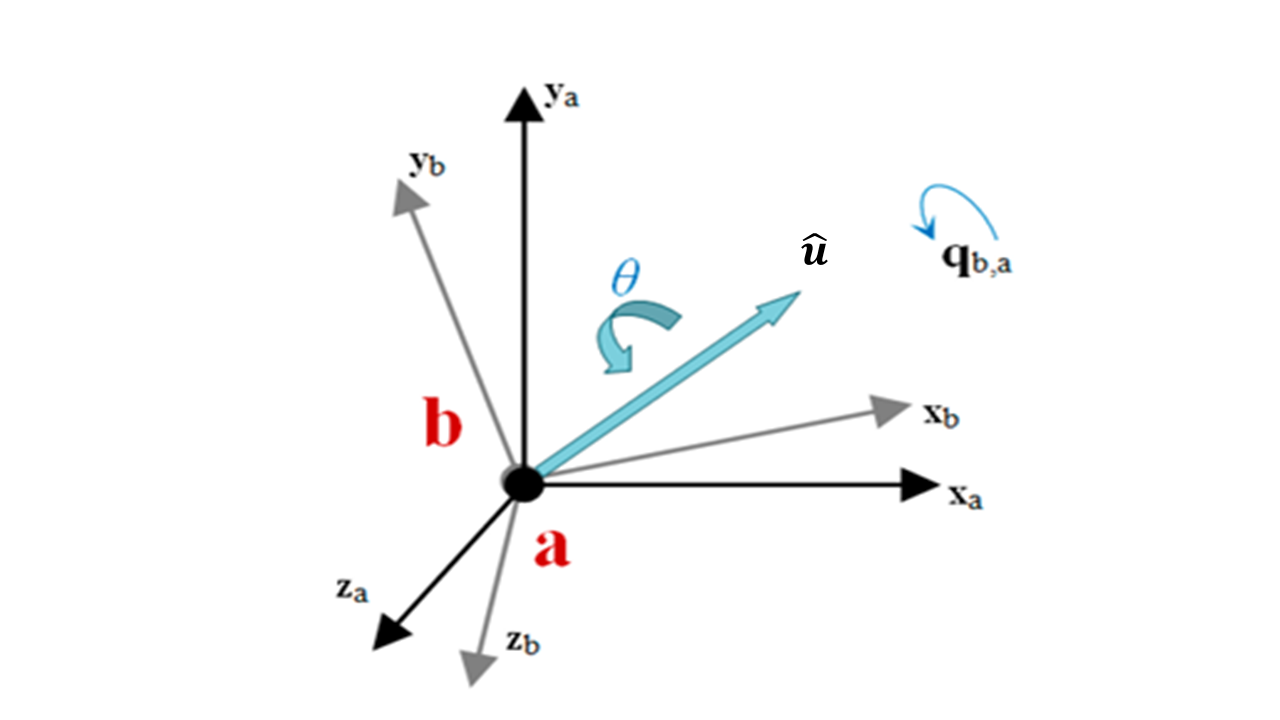
\includegraphics[width=0.5\linewidth]{figures/quad rotation.png}
    \caption{Quaternion representation of rotation along rotation axis $\hat{u}$}
    \label{fig:Quaternion representation of rotation along rotation axis}
\end{figure}
%Since normalized or unit quaternion provides a convenient mathematical notation for representing orientations and rotations of objects in 3D space, the  unit quaternion notion was used to derive Quadrotor model. In unit quaternion, scalar component gives the rotation angle whereas the vector part gives the direction of the rotation axis as shown in Eq.\ref{eqn:quaternion_form}.

%\begin{equation}
%q = (q_0, \vec{q}) = \left( \cos\frac{\theta}{2}, \; \sin\frac{\theta}{2} \, \hat{u} \right)
%\tag{3.1}
%\label{eqn 3.1}
%\end{equation}

%where $\hat{u}$ is a unit vector which is constant, not changing with rotation, and it is formed as 
%\[
%\hat{u} = \frac{\vec{q}}{||\vec{q}||}.
%\]

%Quaternion has its own special set of mathematical operator called \textbf{quaternion product} ‘$\otimes$’, which is extensively used in vector transformation and rotational kinematics. The product between two quaternion $q_a = (q_{0a}, \vec{q}_a)$ and $q_b = (q_{0b}, \vec{q}_b)$, is manipulated as
%\begin{equation}
%q_a \otimes q_b = (q_{0a}, \vec{q}_a) \otimes (q_{0b}, \vec{q}_b) = (q_{0a}q_{0b} - \vec{q}_a \cdot \vec{q}_b, \; q_{0a}\vec{q}_b + q_{0b}\vec{q}_a + \vec{q}_a \times \vec{q}_b)
%\tag{3.2}
%\label{eqn 3.2}
%\end{equation}

%Coordinate transformation between any two different reference frames by using quaternion rotation is computed as\cite{guerrero2017quadrotor}:

%\begin{equation}
%X = q \otimes X' \otimes q^*,
%\tag{3.3a}
%\label{{3.3a}}
%\end{equation}

%where $X$ is the rotated vector and  $X'$ denotes vector to be rotated. Since $q$ is unit norm Quaternion i.e. $||q|| = 1$, its inverse is equal to its conjugate. This is proved as.

%\[
%q^{-1} = \frac{1}{q} = \frac{1}{q} \cdot \frac{q^*}{q^*} = \frac{q^*}{||q||^2} = \frac{q^*}{1^2} = q^*.
%\]

%Hence,

%\begin{equation}
%X = q \otimes X' \otimes q^*
%\tag{3.3b}
%\label{3.3b}
%\end{equation}

%%%%%%%%%%%%%%%%%%%%%%%%%%%%%%%%%%%%%%%
Given their elegant mathematical properties, unit quaternions are employed to derive the quadrotor dynamic model. In the unit quaternion representation shown in Equation~\ref{eqn:quaternion_form}, the scalar component $q_0 = \cos(\theta/2)$ encodes the rotation angle, while the vector component $\vec{q} = \sin(\theta/2)\hat{u}$ specifies the rotation axis direction, where $\hat{u}$ is the unit vector:
\begin{equation}
\hat{u} = \frac{\vec{q}}{\|\vec{q}\|}.
\label{eqn:rotation_axis}
\end{equation}

Quaternions utilize a specialized multiplication operator called the \textbf{quaternion product}, denoted by `$\otimes$', which is fundamental to vector transformations and rotational kinematics. For two quaternions $q_a = (q_{0a}, \vec{q}_a)$ and $q_b = (q_{0b}, \vec{q}_b)$, the product is defined as:
\begin{equation}
q_a \otimes q_b = \left( q_{0a}q_{0b} - \vec{q}_a \cdot \vec{q}_b, \; q_{0a}\vec{q}_b + q_{0b}\vec{q}_a + \vec{q}_a \times \vec{q}_b \right).
\label{eqn:quaternion_product}
\end{equation}

Coordinate transformations between reference frames are performed using quaternion rotation \cite{guerrero2017quadrotor}:
\begin{equation}
X = q \otimes X' \otimes q^*,
\label{eqn:quaternion_rotation}
\end{equation}
where $X'$ is the vector in the original frame, $X$ is the transformed vector, and $q^*$ denotes the quaternion conjugate. For unit quaternions ($\|q\| = 1$), the inverse equals the conjugate, since:
\begin{equation}
q^{-1} = \frac{q^*}{\|q\|^2} = \frac{q^*}{1} = q^*.
\label{eqn:quaternion_inverse}
\end{equation}


%%%%%%%%%%%%%%%%%%%%%%%%%%%%%%%%%%%%%%%%%%%%

%This implies, multiplying two or more rotation quaternion produces another rotation quaternion that represents the total rotation obtained by performing each individual rotation for each quaternion. Vectors can be transformed from one axis system to another if they are first transformed into quaternion with a zero scalar value, also this is known as pure quaternion. This is used to transform the vector coordinate between different rotated reference frames. Since quaternion measures quantities with respect to  IF, quaternion based Rotation matrix that transform quantities from IF to the BF is obtained as.
%\[
%\begin{bmatrix} 0 \\ r_b \end{bmatrix} 
%= q \otimes \begin{bmatrix} 0 \\ r_i \end{bmatrix} \otimes q^*
%\]

%\[
%q \otimes \begin{bmatrix} 0 \\ r_i \end{bmatrix} = [q_0, q_1, q_2, q_3] \otimes [0, x_i, y_i, z_i]
%\]

%\noindent where
%\begin{itemize}
   % \item $q$ : unit quaternion representing orientation
   % \item $q_0$ : scalar part of the quaternion given in Eq. \ref{eqn 3.1}
   % \item $q_1, q_2, q_3$ : vector part of the quaternion given in Eq. \ref{eqn 3.1}
%\end{itemize}

%Let $v_1 = [q_1, q_2, q_3]$, and $v_2 = [x_i, y_i, z_i]$ then by using equation \ref{eqn 3.2} it was found  

%\[
%[q_0, v_1] \otimes [0, v_2] = (q_0 \cdot 0 - v_1 \cdot v_2, \; q_0 v_2 + 0 \cdot v_1 + v_1 \times v_2)
%\]

%\[
%\Rightarrow v_1 \cdot v_2 = [q_1, q_2, q_3] \cdot [x_i, y_i, z_i] = q_1 x_i + q_2 y_i + q_3 z_i
%\]

%\[
%\Rightarrow v_1 \times v_2 = 
%\begin{bmatrix}
%q_1 \\ q_2 \\ q_3
%\end{bmatrix}
%\times
%\begin{bmatrix}
%x_i \\ y_i \\ z_i
%\end{bmatrix}
%=
%\begin{bmatrix}
%q_2 z_i - q_3 y_i \\
%q_3 x_i - q_1 z_i \\
%q_1 y_i - q_2 x_i
%\end{bmatrix}
%\]

%Let $w = (w_0, \vec{w}) = q \otimes \begin{bmatrix} 0 \\ r_i \end{bmatrix}$, where $w_0$ is scalar part and $\vec{w}$ is vector part of Quaternion $w$.

%\[
%w =
%\begin{bmatrix}
%q_0 \cdot 0 - v_1 \cdot v_2 \\
%q_0 v_2 + 0 \cdot v_1 + v_1 \times v_2
%\end{bmatrix}
%=
%\begin{bmatrix}
%-(q_1 x_i + q_2 y_i + q_3 z_i) \\
%q_0 x_i + q_2 z_i - q_3 y_i \\
%q_0 y_i + q_3 x_i - q_1 z_i \\
%q_0 z_i + q_1 y_i - q_2 x_i
%\end{bmatrix}
%\]

%Then, the total rotation is solved by multiplying $w$ with $q^*$:

%\[
%q \otimes \begin{bmatrix} 0 \\ r_i \end{bmatrix} \otimes q^* = w \otimes q^*
%\]

%where $q^* = (q_0, -q_1, -q_2, -q_3) = (q_0, -\vec{q})$.

%By using equation \ref{eqn 3.2}, the two quaternion product is solved as follows:


%%%%%%%%%%%%%%%%%%%%%%%%%%


An important property of quaternions is that the product of two or more rotation quaternions yields another rotation quaternion representing the cumulative effect of applying each individual rotation sequentially. This compositional property makes quaternions particularly efficient for representing complex orientation sequences.To transform vectors between reference frames, they are first expressed as pure quaternions quaternions with zero scalar components. A vector $\bm{r}_i = [x_i, y_i, z_i]^T$ in the inertial frame (IF) is represented as the pure quaternion $(0, \bm{r}_i)$. The transformation to the body frame (BF) is then computed as:
\begin{equation}
\begin{bmatrix} 0 \\ \bm{r}_b \end{bmatrix} 
= q \otimes \begin{bmatrix} 0 \\ \bm{r}_i \end{bmatrix} \otimes q^*,
\label{eqn:quaternion_frame_transform}
\end{equation}
where $q = (q_0, q_1, q_2, q_3)$ is the unit quaternion representing the body orientation relative to the inertial frame, and $q^* = (q_0, -q_1, -q_2, -q_3)$ denotes its conjugate.

%\subsubsection*{Derivation of the Transformation}

The transformation is evaluated through two successive quaternion multiplications.

\paragraph{First multiplication: $w = q \otimes \begin{bmatrix} 0 \\ \bm{r}_i \end{bmatrix}$}

Define the vector components $\bm{v}_1 = [q_1, q_2, q_3]^T$ and $\bm{v}_2 = [x_i, y_i, z_i]^T$. Applying the quaternion product formula (Equation~\ref{eqn:quaternion_product}):
\begin{equation}
(q_0, \bm{v}_1) \otimes (0, \bm{v}_2) = (q_0 \cdot 0 - \bm{v}_1 \cdot \bm{v}_2, \; q_0\bm{v}_2 + 0 \cdot \bm{v}_1 + \bm{v}_1 \times \bm{v}_2),
\end{equation}
which simplifies to:
\begin{equation}
w = (-\bm{v}_1 \cdot \bm{v}_2, \; q_0\bm{v}_2 + \bm{v}_1 \times \bm{v}_2).
\end{equation}

The required dot and cross products are:
\begin{align}
\bm{v}_1 \cdot \bm{v}_2 &= q_1 x_i + q_2 y_i + q_3 z_i, \\
\bm{v}_1 \times \bm{v}_2 &= 
\begin{bmatrix}
q_2 z_i - q_3 y_i \\
q_3 x_i - q_1 z_i \\
q_1 y_i - q_2 x_i
\end{bmatrix}.
\end{align}

Substituting these yields the intermediate quaternion $w = (w_0, \bm{w})$:
\begin{equation}
w = 
\begin{bmatrix}
-(q_1 x_i + q_2 y_i + q_3 z_i) \\
q_0 x_i + q_2 z_i - q_3 y_i \\
q_0 y_i + q_3 x_i - q_1 z_i \\
q_0 z_i + q_1 y_i - q_2 x_i
\end{bmatrix}.
\label{eqn:intermediate_w}
\end{equation}

\paragraph{Second multiplication: $\bm{r}_b^q = w \otimes q^*$}

The final transformation is obtained by multiplying the intermediate quaternion $w$ with the conjugate $q^* = (q_0, -q_1, -q_2, -q_3)$:
\begin{equation}
\begin{bmatrix} 0 \\ \bm{r}_b \end{bmatrix} = w \otimes q^*.
\label{eqn:final_step}
\end{equation}

This second quaternion product, evaluated using Equation~\ref{eqn:quaternion_product}, yields the rotated vector $\bm{r}_b$ in the body frame. The scalar component of the result is zero, confirming that the output is a pure quaternion representing the transformed vector.

%%%%%%%%%%%%%%%%%%%%%%%%%%%%%


%\begin{small}
%\begin{align*}
%w \otimes q^* &= (w_0 q_0 - \vec{w}\cdot \vec{q},\; w_0 \vec{q} + q_0 \vec{w} + \vec{w} \times \vec{q}) \\[1ex]
%\Rightarrow w_0 q_0 &= (-q_1 x_i - q_2 y_i - q_3 z_i) q_0 
%= -q_0 q_1 x_i - q_0 q_2 y_i - q_0 q_3 z_i \\[1ex]
%\Rightarrow \vec{w}\cdot \vec{q} &= (q_0 x_i + q_2 z_i - q_3 y_i,\; 
%q_0 y_i + q_3 x_i - q_1 z_i,\; 
%q_0 z_i + q_1 y_i - q_2 x_i) \cdot (-q_1,-q_2,-q_3) \\[1ex]
%&= -q_0 q_1 x_i - q_0 q_2 y_i - q_0 q_3 z_i
%\end{align*}
%\end{small}

%Hence, the real part becomes  
%\[
%w_0 q_0 - \vec{w}\cdot \vec{q} = -q_0 q_1 x_i - q_0 q_2 y_i - q_0 q_3 z_i + q_0 q_1 x_i + q_0 q_2 y_i + q_0 q_3 z_i = 0
%\]

%\noindent$\bullet \; w_0 \vec{q}$:
%\[
%(-q_1 x_i - q_2 y_i - q_3 z_i)(-q_1,-q_2,-q_3) =
%\begin{bmatrix}
%q_1^2 x_i + q_1 q_2 y_i + q_1 q_3 z_i \\
%q_2 q_1 x_i + q_2^2 y_i + q_2 q_3 z_i \\
%q_3 q_1 x_i + q_3 q_2 y_i + q_3^2 z_i
%\end{bmatrix}
%\]

%\noindent$\bullet \; q_0 \vec{w}$:
%\[
%q_0 \begin{bmatrix}
%q_0 x_i + q_2 z_i - q_3 y_i \\
%q_0 y_i + q_3 x_i - q_1 z_i \\
%q_0 z_i + q_1 y_i - q_2 x_i
%\end{bmatrix}
%=
%\begin{bmatrix}
%q_0^2 x_i + q_0 q_2 z_i - q_0 q_3 y_i \\
%q_0^2 y_i + q_0 q_3 x_i - q_0 q_1 z_i \\
%q_0^2 z_i + q_0 q_1 y_i - q_0 q_2 x_i
%\end{bmatrix}
%\]

%\noindent$\bullet \; \vec{w} \times \vec{q}$:
%{\small
%\[
%\begin{bmatrix}
%q_0 x_i + q_2 z_i - q_3 y_i \\
%q_0 y_i + q_3 x_i - q_1 z_i \\
%q_0 z_i + q_1 y_i - q_2 x_i
%\end{bmatrix}
%\times
%\begin{bmatrix}
%-q_1 \\ -q_2 \\ -q_3
%\end{bmatrix}
%=
%\begin{bmatrix}
%- q_0 q_3 y_i - q_3^2 x_i + q_1 q_3 z_i + q_0 q_2 z_i + q_1 q_2 y_i + q_2^2 x_i \\
%- q_0 q_1 x_i - q_1^2 y_i + q_1 q_2 x_i + q_2 q_3 z_i + q_1 q_3 x_i + q_3^2 y_i \\
%- q_0 q_2 x_i - q_2^2 z_i + q_2 q_3 y_i + q_1 q_2 z_i + q_3 q_1 x_i + q_3^2 z_i
%\end{bmatrix}
%\]
%}

%Then, by combining the bullet equations, we get the vector part of rotation matrix as:

%\begin{align*}
%w \otimes q^* &= 
%\begin{bmatrix}
%q_1^2 x_i + q_1 q_2 y_i + q_1 q_3 z_i \\
%q_1 q_2 x_i + q_2^2 y_i + q_2 q_3 z_i \\
%q_1 q_3 x_i + q_2 q_3 y_i + q_3^2 z_i
%\end{bmatrix}
%+
%\begin{bmatrix}
%q_0^2 x_i + q_0 q_2 z_i - q_0 q_3 y_i \\
%q_0^2 y_i + q_0 q_3 x_i - q_0 q_1 z_i \\
%q_0^2 z_i + q_0 q_1 y_i - q_0 q_2 x_i
%\end{bmatrix} \\[2ex]
%&\quad +
%\begin{bmatrix}
%- q_0 q_3 y_i - q_3^2 x_i + q_1 q_3 z_i + q_0 q_2 z_i + q_1 q_2 y_i + q_2^2 x_i \\
%- q_0 q_1 x_i - q_1^2 y_i + q_1 q_2 x_i + q_2 q_3 z_i + q_1 q_3 x_i + q_3^2 y_i \\
%- q_0 q_2 x_i - q_2^2 z_i + q_2 q_3 y_i + q_1 q_2 z_i + q_3 q_1 x_i + q_3^2 z_i
%\end{bmatrix} \\[2ex]
%&=
%\begin{bmatrix}
%q_1^2 x_i + 2 q_1 q_2 y_i + 2 q_1 q_3 z_i + q_0^2 x_i + 2 q_0 q_2 z_i - 2 q_0 q_3 y_i - q_3^2 x_i - q_2^2 x_i \\
%2 q_1 q_2 x_i + q_2^2 y_i + 2 q_2 q_3 z_i + q_0^2 y_i + 2 q_0 q_3 x_i - 2 q_0 q_1 z_i - q_1^2 y_i - q_3^2 y_i \\
%2 q_1 q_3 x_i + 2 q_2 q_3 y_i + q_3^2 z_i + q_0^2 z_i + 2 q_0 q_1 y_i - 2 q_0 q_2 x_i - q_1^2 z_i - q_2^2 z_i
%\end{bmatrix} \\[2ex]
%&=
%\begin{bmatrix}
%(q_0^2 + q_1^2 - q_2^2 - q_3^2)x_i + 2(q_1 q_2 - q_0 q_3) y_i + 2(q_1 q_3 + q_0 q_2) z_i \\
%2(q_1 q_2 + q_0 q_3)x_i + (q_0^2 - q_1^2 + q_2^2 - q_3^2) y_i + 2(q_2 q_3 - q_0 q_1) z_i \\
%2(q_1 q_3 - q_0 q_2)x_i + 2(q_2 q_3 + q_0 q_1) y_i + (q_0^2 - q_1^2 - q_2^2 + q_3^2) z_i
%\end{bmatrix} \\[2ex]
%&=
%\begin{bmatrix}
%q_0^2 + q_1^2 - q_2^2 - q_3^2 & 2(q_1 q_2 - q_0 q_3) & 2(q_1 q_3 + q_0 q_2) \\
%2(q_1 q_2 + q_0 q_3) & q_0^2 - q_1^2 + q_2^2 - q_3^2 & 2(q_2 q_3 - q_0 q_1) \\
%2(q_1 q_3 - q_0 q_2) & 2(q_2 q_3 + q_0 q_1) & q_0^2 - q_1^2 - q_2^2 + q_3^2
%\end{bmatrix}
%\begin{bmatrix}
%x_i \\ y_i \\ z_i
%\end{bmatrix}
%\end{align*}

%Since we are using unit quaternion to represent the attitude of a Quadrotor, they have the property of unit norm, i.e. 
%\[
%||q||^2 = q_0^2 + q_1^2 + q_2^2 + q_3^2 = 1.
%\]

%So, by utilizing this property we can simplify the above rotation matrix further.Quaternion based rotation matrix which projects IF into BF is expressed in simplified form as:
%\[
%\begin{bmatrix}
%x_b\\ y_b\\ z_b
%\end{bmatrix}
%=
%\begin{bmatrix}
%2(q_0^2+q_1^2)-1 & 2(q_1q_2-q_0q_3) & 2(q_0q_2+q_1q_3)\\
%2(q_1q_2+q_0q_3) & 2(q_0^2+q_2^2)-1 & 2(q_2q_3-q_0q_1)\\
%2(q_1q_3-q_0q_2) & 2(q_2q_3+q_0q_1) & 2(q_0^2+q_3^2)-1
%\end{bmatrix}
%\begin{bmatrix}
%x_i\\ y_i\\ z_i
%\end{bmatrix}
%\]
%%%%%%%%%%%%%%%%%%%%%%%%%%%%
%\subsection*{Derivation of Quaternion Rotation Matrix}

To complete the transformation $\bm{r}_b^q = w \otimes q^*$, we apply the quaternion product formula to $w = (w_0, \bm{w})$ and $q^* = (q_0, -\bm{q})$:
\begin{equation}
w \otimes q^* = (w_0 q_0 - \bm{w} \cdot \bm{q}, \; w_0\bm{q} + q_0\bm{w} + \bm{w} \times \bm{q}),
\label{eqn:final_product}
\end{equation}
where $\bm{q} = [q_1, q_2, q_3]^T$.

%\subsubsection*{Scalar Component (verifies pure quaternion)}

Using $w_0 = -(q_1 x_i + q_2 y_i + q_3 z_i)$ and $\bm{w} = [q_0 x_i + q_2 z_i - q_3 y_i, \; q_0 y_i + q_3 x_i - q_1 z_i, \; q_0 z_i + q_1 y_i - q_2 x_i]^T$:
\begin{align}
w_0 q_0 &= -q_0(q_1 x_i + q_2 y_i + q_3 z_i), \\
\bm{w} \cdot (-\bm{q}) &= -(q_0 x_i + q_2 z_i - q_3 y_i)(-q_1) - (q_0 y_i + q_3 x_i - q_1 z_i)(-q_2) \nonumber \\
&\quad - (q_0 z_i + q_1 y_i - q_2 x_i)(-q_3) \nonumber \\
&= q_0(q_1 x_i + q_2 y_i + q_3 z_i).
\end{align}

Therefore, the scalar part vanishes,confirming the result is a pure quaternion:
\begin{equation}
w_0 q_0 - \bm{w} \cdot \bm{q} = 0,
\end{equation}


%\subsubsection*{Vector Component}

The vector part comprises three terms: $w_0(-\bm{q}) + q_0\bm{w} + \bm{w} \times (-\bm{q})$.

\paragraph{Term 1: $w_0(-\bm{q})$}
\begin{equation}
w_0(-\bm{q}) = -(q_1 x_i + q_2 y_i + q_3 z_i)
\begin{bmatrix}
-q_1 \\ -q_2 \\ -q_3
\end{bmatrix}
=
\begin{bmatrix}
q_1^2 x_i + q_1 q_2 y_i + q_1 q_3 z_i \\
q_1 q_2 x_i + q_2^2 y_i + q_2 q_3 z_i \\
q_1 q_3 x_i + q_2 q_3 y_i + q_3^2 z_i
\end{bmatrix}.
\end{equation}

\paragraph{Term 2: $q_0\bm{w}$}
\begin{equation}
q_0\bm{w} = q_0
\begin{bmatrix}
q_0 x_i + q_2 z_i - q_3 y_i \\
q_0 y_i + q_3 x_i - q_1 z_i \\
q_0 z_i + q_1 y_i - q_2 x_i
\end{bmatrix}
=
\begin{bmatrix}
q_0^2 x_i + q_0 q_2 z_i - q_0 q_3 y_i \\
q_0^2 y_i + q_0 q_3 x_i - q_0 q_1 z_i \\
q_0^2 z_i + q_0 q_1 y_i - q_0 q_2 x_i
\end{bmatrix}.
\end{equation}

\paragraph{Term 3: $\bm{w} \times (-\bm{q})$}
\begin{equation}
\bm{w} \times (-\bm{q}) =
\begin{bmatrix}
q_0 x_i + q_2 z_i - q_3 y_i \\
q_0 y_i + q_3 x_i - q_1 z_i \\
q_0 z_i + q_1 y_i - q_2 x_i
\end{bmatrix}
\times
\begin{bmatrix}
-q_1 \\ -q_2 \\ -q_3
\end{bmatrix}
=
\begin{bmatrix}
q_2^2 x_i + q_1 q_2 y_i + q_1 q_3 z_i - q_3^2 x_i + q_0 q_2 z_i - q_0 q_3 y_i \\
q_1 q_2 x_i + q_3^2 y_i + q_2 q_3 z_i - q_1^2 y_i + q_1 q_3 x_i - q_0 q_1 z_i \\
q_1 q_3 x_i + q_2 q_3 y_i + q_3^2 z_i - q_2^2 z_i + q_0 q_1 y_i - q_0 q_2 x_i
\end{bmatrix}.
\end{equation}

%\subsubsection*{Combined Vector Part}

Summing the three terms and collecting coefficients of $x_i$, $y_i$, and $z_i$:
\begin{equation}
\bm{r}_b = 
\begin{bmatrix}
(q_0^2 + q_1^2 - q_2^2 - q_3^2)x_i + 2(q_1 q_2 - q_0 q_3)y_i + 2(q_1 q_3 + q_0 q_2)z_i \\
2(q_1 q_2 + q_0 q_3)x_i + (q_0^2 - q_1^2 + q_2^2 - q_3^2)y_i + 2(q_2 q_3 - q_0 q_1)z_i \\
2(q_1 q_3 - q_0 q_2)x_i + 2(q_2 q_3 + q_0 q_1)y_i + (q_0^2 - q_1^2 - q_2^2 + q_3^2)z_i
\end{bmatrix}.
\end{equation}

This can be expressed in matrix form as:
\begin{equation}
\bm{r}_b = R_q^{i \to b} \bm{r}_i,
\label{eqn:rotation_matrix_form}
\end{equation}
where:
\begin{equation}
R_q^{i \to b} =
\begin{bmatrix}
q_0^2 + q_1^2 - q_2^2 - q_3^2 & 2(q_1 q_2 - q_0 q_3) & 2(q_1 q_3 + q_0 q_2) \\
2(q_1 q_2 + q_0 q_3) & q_0^2 - q_1^2 + q_2^2 - q_3^2 & 2(q_2 q_3 - q_0 q_1) \\
2(q_1 q_3 - q_0 q_2) & 2(q_2 q_3 + q_0 q_1) & q_0^2 - q_1^2 - q_2^2 + q_3^2
\end{bmatrix}.
\label{eqn:rotation_matrix_general}
\end{equation}

\subsubsection*{Simplified Form Using Unit Quaternion Property}

For unit quaternions, $\|q\|^2 = q_0^2 + q_1^2 + q_2^2 + q_3^2 = 1$. This allows simplification of the diagonal elements:
\begin{align}
q_0^2 + q_1^2 - q_2^2 - q_3^2 &= q_0^2 + q_1^2 - (1 - q_0^2 - q_1^2) = 2(q_0^2 + q_1^2) - 1, \\
q_0^2 - q_1^2 + q_2^2 - q_3^2 &= q_0^2 + q_2^2 - (1 - q_0^2 - q_2^2) = 2(q_0^2 + q_2^2) - 1, \\
q_0^2 - q_1^2 - q_2^2 + q_3^2 &= q_0^2 + q_3^2 - (1 - q_0^2 - q_3^2) = 2(q_0^2 + q_3^2) - 1.
\end{align}

Therefore, the quaternion-based rotation matrix from IF to BF simplifies to:
\begin{equation}
%\boxed{
\begin{bmatrix}
x_b \\ y_b \\ z_b
\end{bmatrix}
=
\begin{bmatrix}
2(q_0^2 + q_1^2) - 1 & 2(q_1 q_2 - q_0 q_3) & 2(q_1 q_3 + q_0 q_2) \\
2(q_1 q_2 + q_0 q_3) & 2(q_0^2 + q_2^2) - 1 & 2(q_2 q_3 - q_0 q_1) \\
2(q_1 q_3 - q_0 q_2) & 2(q_2 q_3 + q_0 q_1) & 2(q_0^2 + q_3^2) - 1
\end{bmatrix}
\begin{bmatrix}
x_i \\ y_i \\ z_i
\end{bmatrix}
%}
\label{eqn:rotation_matrix_simplified}
\end{equation}



%%%%%%%%%%%%%%%%%%%%%%%%%%

Even though thrust generated from each propeller is measured with respect to BF, Newton laws are valid on IF only. Hence, we need the rotation matrix that projects BF into IF. Since the rotation matrix is orthogonal (determinant \(\pm1\)), the inverse equals its transpose. Therefore, the rotation matrix which projects the BF quantities into IF now becomes:
\begin{equation}
\label{eq:R_ib}
\begin{bmatrix}
x_i\\ y_i\\ z_i
\end{bmatrix}
=
\begin{bmatrix}
2(q_0^2+q_1^2)-1 & 2(q_1q_2+q_0q_3) & 2(q_1q_3-q_0q_2)\\
2(q_1q_2-q_0q_3) & 2(q_0^2+q_2^2)-1 & 2(q_2q_3+q_0q_1)\\
2(q_1q_3+q_0q_2) & 2(q_2q_3-q_0q_1) & 2(q_0^2+q_3^2)-1
\end{bmatrix}
\begin{bmatrix}
x_b\\ y_b\\ z_b
\end{bmatrix}
%\tag{3.4}
\label{eqn 3.4}
\end{equation}

Compared to the Euler rotation matrix the quaternion rotation matrix in \eqref{eqn 3.4} is more compact, efficient, and numerically stable. Relationship between axis angle representation \(\theta\) (shown in Figure\ref{fig:Rigid Body rotation}) and quaternion, derived from Eqn. \eqref{eqn:quaternion_form} and the exponential map, is:
\[
q=(q_0,\vec q)=\Big(\cos\frac{\theta}{2},\,\sin\frac{\theta}{2}\,\hat u\Big)
= \exp\!\big(\,\bar\theta\,\hat u\,\big),
\]
with
\begin{equation}
\bar{\theta}=2\ln q.
%\tag{3.5}
\label{3.5}
\end{equation}

%\begin{figure}[h!]
    %\centering
   % 
\includegraphics[width=0.5\linewidth]{Figures/Rigid Body rotation.PNG}
    %\caption{Rigid body rotation in terms of axis-angle notation\cite{guerrero2017quadrotor}}
    %\label{fig:Rigid Body rotation}
%\end{figure}

\begin{figure}[h!]
    \centering
    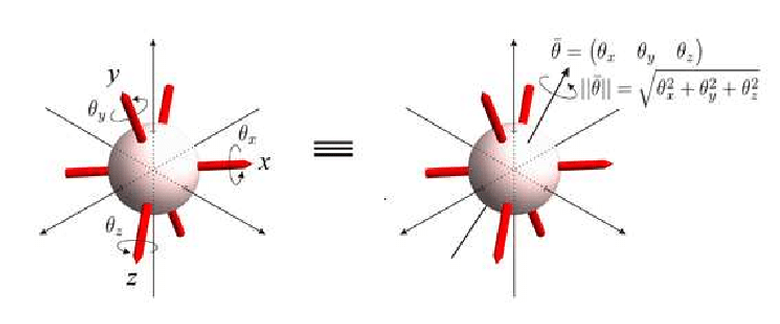
\includegraphics[width=0.5\linewidth]{figures/Rigid Body rotation.PNG}

    % Caption for List of Figures (no citation)
    \caption{Rigid body rotation in terms of axis-angle notation} \cite{guerrero2017quadrotor}

    % Caption shown only below the figure (with citation)
    %\caption*{Source: \cite{guerrero2017quadrotor}}

    \label{fig:Rigid Body rotation}
\end{figure}


And to get body frame velocity $\omega$ let’s take derivative of equation \eqref{3.5} from both sides:

\[
\omega = \frac{d\bar{\theta}}{dt} = \frac{d}{dt}(2 \ln q) 
= 2 \cdot \frac{1}{q} \otimes \dot{q} = 2 q^{-1} \otimes \dot{q}
\]

%\[
%\omega = 2 q^{-1} \otimes \dot{q}
%\]

Then by multiplying both sides with $\tfrac{1}{2}q$, and taking its derivative we have:

\begin{equation}
\dot{q} = \tfrac{1}{2} q \otimes \omega = \tfrac{1}{2} \big[ (q_0, \vec{q}) \otimes (0, \omega) \big] = \tfrac{1}{2} \big[ (q_0 \ast 0 - \vec{q}\cdot \omega,\; q_0 \ast \omega + 0 \ast \vec{q} + \vec{q} \times \omega ) \big]
%\tag{3.6}
\label{3.6}
\end{equation}

%By using equation \eqref{eqn:quaternion_product}, derivative of quaternion in equation \eqref{3.6} can be expanded as:
%\[
%\dot{q} = (\dot{q}_0, \dot{\vec{q}}) 
%= \tfrac{1}{2} q \otimes \omega 
%= \tfrac{1}{2} \big[ (q_0, \vec{q}) \otimes (0, \omega) \big] 
%\]

%\[
%(\dot{q}_0, \dot{\vec{q}}) 
%= \tfrac{1}{2} \big[ (q_0 \ast 0 - \vec{q}\cdot \omega,\; q_0 \ast \omega + 0 \ast \vec{q} + \vec{q} \times \omega ) \big]
%\]

% Force equation counter to 11 so next is 3.12
%\setcounter{equation}{6}


%\[
\begin{equation}
\dot{q}_0 = -\frac{1}{2}\,\vec{q}\cdot \omega \\
\dot{\vec{q}} = \frac{1}{2}\left(q_0\omega + \vec{q}\times\omega\right)
\label{3.7}
\end{equation}

%\end{cases}
%\]




Where $\,\omega=[p,q,r]^{T}\,$ is angular velocity in BF.

By expanding equation \eqref{3.7}, we can obtain the following equations for quaternion rates:

%\[\dot q_0=-\tfrac{1}{2}\big([q_1,q_2,q_3]\!\cdot\![p,q,r]\big)
%= -\tfrac{1}{2}\,(p q_1+q q_2+r q_3)\]

%\[
%\dot{\vec q}=\tfrac{1}{2}\,(q_0\omega+\vec q\times\omega)
%=\tfrac{1}{2}\!\left(
%\begin{bmatrix} q_0 \\[2pt] q_0 \\[2pt] q_0 \end{bmatrix}\!\odot\!\begin{bmatrix} p\\ q\\ r \end{bmatrix}
%+\begin{bmatrix} q_1\\ q_2\\ q_3 \end{bmatrix}\!\times\!\begin{bmatrix} p\\ q\\ r \end{bmatrix}
%\right)
%=\tfrac{1}{2}\!\left(
%\begin{bmatrix} p q_0\\ q q_0\\ r q_0 \end{bmatrix}
%+
%\begin{bmatrix} r q_2-q q_3\\ p q_3-r q_1\\ q q_1-p q_2 \end{bmatrix}
%\right)
%=\tfrac{1}{2}
%\begin{bmatrix}
%p q_0+r q_2-q q_3\\
%q q_0+p q_3-r q_1\\
%r q_0+q q_1-p q_2
%\end{bmatrix}\]

%\[\dot q_0=-\tfrac{1}{2}\big([q_1,q_2,q_3]\!\cdot\![p,q,r]\big)
%= -\tfrac{1}{2}\,(p q_1+q q_2+r q_3)\]
\begin{small}
    \[
\dot{\vec q}=\tfrac{1}{2}\,(q_0\omega+\vec q\times\omega)
=\tfrac{1}{2}\!\left(
\begin{bmatrix} q_0 \\[2pt] q_0 \\[2pt] q_0 \end{bmatrix}\!\odot\!\begin{bmatrix} p\\ q\\ r \end{bmatrix}
+\begin{bmatrix} q_1\\ q_2\\ q_3 \end{bmatrix}\!\times\!\begin{bmatrix} p\\ q\\ r \end{bmatrix}
\right)
=\tfrac{1}{2}\!\left(
\begin{bmatrix} p q_0\\ q q_0\\ r q_0 \end{bmatrix}
+
\begin{bmatrix} r q_2-q q_3\\ p q_3-r q_1\\ q q_1-p q_2 \end{bmatrix}
\right)
=\tfrac{1}{2}
\begin{bmatrix}
p q_0+r q_2-q q_3\\
q q_0+p q_3-r q_1\\
r q_0+q q_1-p q_2
\end{bmatrix}
\]

\end{small}



Hence, relation between quaternion rates and BF angular velocities is summarized as
\begin{equation}
\begin{bmatrix}
\dot q_0\\ \dot q_1\\ \dot q_2\\ \dot q_3
\end{bmatrix}
=\tfrac{1}{2}
\begin{bmatrix}
 q_0 & -q_1 & -q_2 & -q_3\\
 q_1 &  q_0 & -q_3 &  q_2\\
 q_2 &  q_3 &  q_0 & -q_1\\
 q_3 & -q_2 &  q_1 &  q_0
\end{bmatrix}
\begin{bmatrix}
0\\ p\\ q\\ r
\end{bmatrix}
%\tag{3.8}
\label{3.8}
\end{equation}


Where : 
\begin{equation}
\begin{bmatrix}
p \\ q \\ r
\end{bmatrix}
=
\begin{bmatrix}
1 & 0 & -s_\theta \\
0 & c_\phi & s_\phi c_\theta \\
0 & -s_\phi & c_\phi c_\theta
\end{bmatrix}
\begin{bmatrix}
\dot{\phi} \\ \dot{\theta} \\ \dot{\psi}
\end{bmatrix}
%\tag{3.8a}
\label{3.8a}
\end{equation}

\subsection{Mathematical Modeling of Quadrotor Dynamics}

%Since almost all systems in real life are nonlinear in nature, Control Engineers design either linear controller by linearizing those nonlinear systems at some operating point; or they design nonlinear controller based on simplified nonlinear model of the system by ignoring some features which are assumed to have less effect on the system. During simulation, the designed controller may show promising results by effectively driving tracking error toward zero. However, when we implement the developed control algorithm in the real system, the error may be diverged rather than converged toward zero. This is due to the designed control law, which is designed based on linearized/simplified model not based on the real plant, so unmodeled dynamics, which are neglected during modeling, may decrease controller performance and also they may cause the system unstable. 

Most real world systems are inherently nonlinear. Control engineers address this challenge through two primary approaches: designing linear controllers by linearizing the nonlinear system at an operating point, or developing nonlinear controllers based on simplified models that omit features with negligible effects. Although simulations typically show excellent performance with tracking errors converging to zero, implementation on actual systems often reveals divergent error behavior. This performance gap occurs because controllers are designed using linearized or simplified models rather than the true plant dynamics. The unmodeled dynamics, neglected during model development, can substantially reduce controller effectiveness and may even cause system instability. To mitigate the adverse effects of unmodeled dynamics, this section introduces a more realistic representation of the quadrotor system by incorporating all factors that significantly influence its dynamic behavior. This approach is motivated by a fundamental principle in control engineering, improving the accuracy of the system model generally enhances controller performance, even though it may increase the overall complexity of the model.

%To solve such harmful effect of unmodeled dynamics, in this section more realistical behavior of Quadrotor is enforced by considering every effect which has significant effect on the Quadrotor dynamics. This point is raised from general fact of Control Engineering arena which is when we design the model more accurately, controller performance will be increased though complexity of the model is increased.% As we will see later, due to high generalization capability of ANN, designed complex system model will be first represented by ANN model via system identification process; then based on the estimated model controller will be designed.

\bigskip

In order to derive mathematical model of Quadrotor dynamics, it is important to take the following assumptions \cite{doukhi2017intelligent},\cite{baoying2020research}, Structure of the Quadrotor is rigid with constant mass and uniform symmetry, gravitational force doesn’t change with altitude,quadrotor center of mass coincides with its geometric center,the resistance and inductance of BLDC motor are negligible, and at hovering position velocity of air and propellers are equal.

%\begin{enumerate}
   % \item Structure of the Quadrotor is rigid with constant mass and uniform symmetry,
   % \item Gravitational force doesn’t change with altitude,
   % \item Quadrotor center of mass coincides with its geometric center,
    %\item The resistance and inductance of BLDC motor are negligible, and
   % \item At hovering position velocity of air and propellers are equal.
%\end{enumerate}

\noindent
%Since Quadrotor structure is assumed to be rigid body, we can use Newtons laws to derive its dynamics. In the following subsections mathematical model of Quadrotor will be derived first by applying Newton-Euler approach and Newton-Quaternion approach for fully actuated rotational and underactuated translational dynamics based on Free Body Diagram (FBD) of Quadrotor as shown in figure\ref{fig:Quadrotor free body diagram}. Then, by comparing the two approaches, the best of the two approaches will be taken to develop appropriate model for realtime implementation and to enhance controller performance.

Since the quadrotor structure is assumed to behave as a rigid body, its dynamics can be derived using Newton’s laws of motion. In the following subsections, the mathematical model of the quadrotor is developed using the Newton--Quaternion approach to represent the system dynamics. This formulation is used to describe the fully actuated rotational dynamics and the underactuated translational dynamics based on the free body diagram (FBD) of the quadrotor shown in Figure~\ref{fig:Quadrotor free body diagram}. The quaternion-based representation provides an effective framework for modeling the quadrotor attitude dynamics and is suitable for real-time implementation and improved controller performance.



\subsubsection{Quadrotor Rotational Motion}

%By using Newton $2^{nd}$ law of rotational motion for fully actuated Quadrotor rotational dynamics, the net moment derived from BF as follows:
By applying Newton's $2^{\text{nd}}$ law of rotational motion to the fully actuated rotational dynamics of the quadrotor, the resultant moment acting on the system can be derived from the body frame (BF) as follows:

\begin{equation}
\sum \tau_i = J \alpha = [U_2, U_3, U_4]^T - M_{gyro} - M_{aero}
%\tag{3.9}
\label{3.9}
\end{equation}

Where: $J =$ inertia matrix. 
$\alpha = [\dot{p}, \dot{q}, \dot{r}]^T$ are angular accelerations in BF; 
$U_2, U_3,$ and $U_4$ are moments on BF which are used to control roll, pitch, and yaw, respectively; 
$M_{gyro} =$ gyroscopic moment, and 
$M_{aero} =$ aerodynamic frictional moment.

\paragraph{Inertia Matrix of the Quadrotor}

%\subsubsubsection{Inertia Matrix of the Quadrotor}
%Actual inertia matrix of Quadrotor is assumed to be constant matrix,
%since structure of a Quadrotor is assumed to be symmetrical with respect to coordinate system, 
%$J_{xy} = J_{xz} = J_{yz} = 0$ and $J_{xx} = J_{yy}$~\cite{beard2008quadrotor}. 
%Hence, inertia matrix for Quadrotor now becomes a diagonal matrix. Where: $J_{xx}, J_{yy},$ and $J_{zz}$ are moments of inertia about the principal axis on the BF.
The inertia matrix of the quadrotor is assumed to be constant. Since the quadrotor structure is considered symmetric with respect to the coordinate axes, the products of inertia satisfy $J_{xy}=J_{xz}=J_{yz}=0$, and the moments of inertia about the $x$ and $y$ axes are equal, i.e., $J_{xx}=J_{yy}$~\cite{beard2008quadrotor}. Consequently, the inertia matrix of the quadrotor reduces to a diagonal form. Here, $J_{xx}$, $J_{yy}$, and $J_{zz}$ represent the moments of inertia about the principal axes of the body frame (BF).

\begin{equation}
J =
\begin{bmatrix}
J_{xx} & -J_{xy} & -J_{xz} \\
-J_{xy} & J_{yy} & -J_{yz} \\
-J_{xz} & -J_{yz} & J_{zz}
\end{bmatrix} J =
\begin{bmatrix}
J_{xx} & 0 & 0 \\
0 & J_{yy} & 0 \\
0 & 0 & J_{zz}
\end{bmatrix}
%\tag{3.10}
\label{3.10} 
\end{equation}
%\[

%\]



%Since structure of a Quadrotor is assumed to be symmetrical with respect to coordinate system, 
%$J_{xy} = J_{xz} = J_{yz} = 0$ and $J_{xx} = J_{yy}$~\cite{beard2008quadrotor}. 
%Hence, inertia matrix for Quadrotor now becomes a diagonal matrix:

%\begin{equation}
%J =
%\begin{bmatrix}
%J_{xx} & 0 & 0 \\
%0 & J_{yy} & 0 \\
%0 & 0 & J_{zz}
%\end{bmatrix}
%\tag{3.10}
%\label{3.10}
%\end{equation}

%Where: $J_{xx}, J_{yy},$ and $J_{zz}$ are moments of inertia about the principal axis on the BF.

\paragraph*{Euler’s Equations of Rigid Body Dynamics}

%Euler’s rotation equations is a vector quasi-linear first order ordinary differential equation which describe the rotation of a Quadrotor in BF w.r.t IF. Let the unit vectors $\vec{i}, \vec{j},$ or $\vec{k}$ representing standard basis of unit vectors in the rotating BF. If they are rotating at the speed of $\omega$ w.r.t fixed IF, then time derivative of each rotating coordinate frame: $\vec{i}, \vec{j},$ or $\vec{k}$ of unit vector $\vec{u}$ becomes:

Euler's rotational equations form a vector quasi-linear first-order ordinary differential equation that describes the rotational motion of a quadrotor in the body frame (BF) with respect to the inertial frame (IF). Let the unit vectors $\vec{i}$, $\vec{j}$, and $\vec{k}$ denote the standard basis vectors of the rotating body frame. If the body frame rotates with an angular velocity $\omega$ relative to the fixed inertial frame, then the time derivative of each rotating unit vector $\vec{i}$, $\vec{j}$, and $\vec{k}$, represented generically by the unit vector $\vec{u}$, can be expressed as follows:


\begin{equation}
    \frac{d}{dt}\vec{u} = \omega \times \vec{u}
\end{equation}



%Since both angular acceleration and angular velocity of Quadcopter are vector quantities, both their magnitudes and directions in rotating BF are change in with time w.r.t fixed IF. Therefore, by using chain rule we have the following expression for net moment of Quadrotor:

Since the angular velocity and angular acceleration of the quadrotor are vector quantities, their magnitudes and directions in the rotating body frame (BF) vary with time relative to the inertial frame (IF). Therefore, by applying the chain rule, the net moment of the quadrotor can be expressed as follows:

%\[
\begin{equation}
J\alpha = J \frac{d}{dt}(\omega \vec{u}) 
= J \frac{d\omega}{dt}\vec{u} + \frac{d}{dt}(J\omega \vec{u})
= J \frac{d\omega}{dt}\vec{u} + \omega \times (J\omega \vec{u})
= J \frac{d\omega}{dt} + \omega \times (J\omega) = J\dot{\omega} + \omega \times (J\omega)
\label{3.11}
\end{equation}

%\]

%\begin{equation}
%J\alpha = J\dot{\omega} + \omega \times (J\omega)
%\tag{3.11}
%\label{3.11}
%\end{equation}

%Where: $\omega = \omega \vec{u} = [p, q, r]^T$ which represents Euler angular rates in Quadrotor BF.



\subsubsection{Gyroscopic Effect of Propellers}

The spinning propellers induces a gyroscopic torque when the Quad rotates in the space~\cite{selfridge2014multivariable}.
This induced torque act on the axis which is perpendicular to stationary axes of propellers rotation
and axes of Quad body rotation along x-axis or y-axis, and it is expressed as:

\begin{equation}
    M_{gyro} = J_p \Omega \times \omega
    %\tag{3.12}
    \label{3.12}
\end{equation}

Where $\omega$ is speed of Quad body rotates along x or y axis, $\Omega$ is angular speed of propellers,
and $J_p$ is inertia of propeller. Since a Quad has four propellers or rotors, we need to solve the
gyro induced torque separately four times along x-axis and four times along y-axis. Based on
Figure~\ref{fig:Quadrotor free body diagram} propeller 2 and 4 rotates in CCW direction, and 1 and 3 in CW direction, the resultant
gyroscopic moment along x-axis: $M_{x_{gyro}}$, and y-axis: $M_{y_{gyro}}$ expressed as follows:

\begin{equation}
    M_{x_{gyro}} = J_p q \Omega_r %\tag{3.13}
    \label{3.13}
\end{equation}

\begin{equation}
    M_{y_{gyro}} = -J_p p \Omega_r %\tag{3.14}
    \label{3.14}
\end{equation}

Where: $\Omega_r = -\Omega_1 + \Omega_2 - \Omega_3 + \Omega_4$ is the net angular velocity of the
propellers and $\Omega_i$ ($i=1,2,3,4$) is velocity of each propeller. Equation~\eqref{3.13} implies that
induced torque about x-axis due to angular rate of change to pitch $q$, i.e. a Quad will feel a body
roll-induced torque when it pitches; this is due to the gyroscopic effect of the four propellers.
The same thing is expressed in Equation~\eqref{3.14} for y-axis induced gyroscopic torque. Rotation about
z-axis contributes no gyroscopic effect from the propellers rotation because the axis of propellers
rotation and vehicle rotation axis pointing in the same direction, so the cross product becomes zero,
i.e., no torque is induced during yaw or z-axis rotation.

\subsubsection{Aerodynamic Effects due to Propellers Rotation}

This is also known as viscous frictional torque in BF resulting from aerodynamic friction, 
and it’s given as~\cite{bensalah2019full}:

\begin{equation}
    M_{aero} = C_a \omega %\tag{3.15}
    \label{3.15}
\end{equation}

% --- context line above the derivation (optional) ---
Where $C_a$ is an aerodynamic coefficient depending on air density and the angular speed of the
quadrotor $\omega$.

By substituting equation \eqref{3.11}-\eqref{3.15} in Eq.\eqref{3.9}, rotational dynamics of Quadrotor is
derived as follows:
\begin{small}
\begin{equation}
\begin{align*}
J \alpha &= [U_2, U_3, U_4]^T - M_{gyro} - M_{aero} \\[6pt]
J\dot{\omega} + \omega \times (J\omega) &= [U_2, U_3, U_4]^T - M_{gyro} - M_{aero} \\[6pt]
\dot{\omega} &= J^{-1} \Big( [U_2, U_3, U_4]^T - \omega \times (J\omega) - M_{gyro} - M_{aero} \Big)
\end{align*} 
\end{equation}


%\begin{align*}
%J \alpha &= [U_2, U_3, U_4]^T - M_{gyro} - M_{aero} \\[6pt]
%J\dot{\omega} + \omega \times (J\omega) &= [U_2, U_3, U_4]^T - M_{gyro} - M_{aero} \\[6pt]
%\dot{\omega} &= J^{-1} \Big( [U_2, U_3, U_4]^T - \omega \times (J\omega) - M_{gyro} - M_{aero} \Big)
%\end{align*}

\begin{align*}
\begin{bmatrix} \dot{p} \\ \dot{q} \\ \dot{r} \end{bmatrix}
&=
\begin{bmatrix}
J_{xx} & 0 & 0 \\
0 & J_{yy} & 0 \\
0 & 0 & J_{zz}
\end{bmatrix}^{-1}
\left(
\begin{bmatrix} U_2 \\ U_3 \\ U_4 \end{bmatrix}
-
\begin{bmatrix} p \\ q \\ r \end{bmatrix}
\times
\begin{bmatrix}
J_{xx} & 0 & 0 \\
0 & J_{yy} & 0 \\
0 & 0 & J_{zz}
\end{bmatrix}
\begin{bmatrix} p \\ q \\ r \end{bmatrix}
-
\begin{bmatrix}
J_p q \Omega_r - C_a p \\
- J_p p \Omega_r - C_a q \\
C_a r
\end{bmatrix}
%\right) \\[8pt]
%&=
%\begin{bmatrix}
%\frac{1}{J_{xx}} & 0 & 0 \\
%0 & \frac{1}{J_{yy}} & 0 \\
%0 & 0 & \frac{1}{J_{zz}}
%\end{bmatrix}
%\left(
%\begin{bmatrix} U_2 \\ U_3 \\ U_4 \end{bmatrix}
%-
%\begin{bmatrix} p \\ q \\ r \end{bmatrix}
%\times
%\begin{bmatrix}
%J_{xx}p \\ J_{yy}q \\ J_{zz}r
%\end{bmatrix}
%-
%\begin{bmatrix}
%J_p q \Omega_r + C_a p \\
%- J_p p \Omega_r + C_a q \\
%C_a r
%\end{bmatrix}
%\right) \\[8pt]
%&=
%\begin{bmatrix}
%\frac{1}{J_{xx}} & 0 & 0 \\
%0 & \frac{1}{J_{yy}} & 0 \\
%0 & 0 & \frac{1}{J_{zz}}
%\end{bmatrix}
%\left(
%\begin{bmatrix} U_2 \\ U_3 \\ U_4 \end{bmatrix}
%-
%\begin{bmatrix}
%(J_{zz}-J_{yy})qr \\
%(J_{xx}-J_{zz})pr \\
%(J_{yy}-J_{xx})pq
%\end{bmatrix}
%-
%\begin{bmatrix}
%J_p q \Omega_r + C_a p \\
%- J_p p \Omega_r + C_a q \\
%C_a r
%\end{bmatrix}
%\right) \\[8pt]
%&=
%\begin{bmatrix}
%\frac{1}{J_{xx}}\left( U_2 + (J_{yy}-J_{zz})qr - J_p q \Omega_r - C_a p \right) \\[6pt]
%\frac{1}{J_{yy}}\left( U_3 + (J_{zz}-J_{xx})pr + J_p p \Omega_r - C_a q \right) \\[6pt]
%\frac{1}{J_{zz}}\left( U_4 + (J_{xx}-J_{yy})pq - C_a r \right)
%\end{bmatrix}
\end{align*}

    
\end{small}



Hence,
% Set counter so next equation is 3.20
%\setcounter{equation}{19}

%\begin{subequations}
%\begin{empheq}[left=\empheqlbrace]{align}
%\dot{p} &= \tfrac{1}{J_{xx}} U_2
       % + \tfrac{J_{yy}-J_{zz}}{J_{xx}} qr
       % - \tfrac{J_p}{J_{xx}} q \Omega_r
        %- \tfrac{C_{a_p}}{J_{xx}} p \label{eq:320a}\\[1.1ex]
%\dot{q} &= \tfrac{1}{J_{yy}} U_3
        %+ \tfrac{J_{zz}-J_{xx}}{J_{yy}} pr
       % + \tfrac{J_p}{J_{yy}} p \Omega_r
       % - \tfrac{C_{a_q}}{J_{yy}} q \label{eq:320b}\\[1.1ex]
%\dot{r} &= \tfrac{1}{J_{zz}} U_4
       % + \tfrac{J_{xx}-J_{yy}}{J_{zz}} pq
       % - \tfrac{C_{a_r}}{J_{zz}} r \label{eq:320c}
%\end{empheq}
%\end{subequations}


\begin{equation}
\left\{
\begin{aligned}
\dot{p} &= \frac{1}{J_{xx}} U_2 
        + \frac{J_{yy}-J_{zz}}{J_{xx}}\, q r
        - \frac{J_p}{J_{xx}}\, q \Omega_r
        - \frac{C_{ap}}{J_{xx}}\, p, \\[6pt]
\dot{q} &= \frac{1}{J_{yy}} U_3
        + \frac{J_{zz}-J_{xx}}{J_{yy}}\, p r
        + \frac{J_p}{J_{yy}}\, p \Omega_r
        - \frac{C_{aq}}{J_{yy}}\, q, \\[6pt]
\dot{r} &= \frac{1}{J_{zz}} U_4
        + \frac{J_{xx}-J_{yy}}{J_{zz}}\, p q
        - \frac{C_{ar}}{J_{zz}}\, r
\end{aligned}
\right.
%\tag{3.16}
\end{equation}



\subsubsection{Quadrotor Translational Motion}

%Translational dynamics of Quadrotor is derived based on Newton 2\textsuperscript{nd} law of translational motion. Since Newton’s laws are valid only in IF, we use the rotation matrix which project thrust force that generated in BF into IF. In these scenario, translational dynamics of Quadrotor is derived in the following sub subsection based on Newton–Euler formalism and Newton–Quaternion formalism as follows:

Translational dynamics of Quadrotor is derived based on Newton 2\textsuperscript{nd} law of translational
motion. Since Newton’s laws are valid only in IF, we use the rotation matrix which project thrust
force that generated in BF into IF. In these scenario, translational dynamics of Quadrotor is derived
in  Newton–Quaternion formalism as follows:




\subsubsubsection{\textbf{Newton--Quaternion Formalism}}

By applying Newton--Quaternion approach, Quadrotor translational dynamics is derived as:
\begin{small}
\begin{equation}
    a = \frac{1}{m}\big[ R_b^{e} U_1 - F_g - F_d \big]
    \label{eq:translation dynamics}
\end{equation}

 Substituting Eqn \eqref{eqn 3.4}, gravity and drag forces  in Eqn \eqref{eq:translation dynamics} it is found to be:
%\[
%\begin{bmatrix}
%\ddot{x} \\[6pt]
%\ddot{y} \\[6pt]
%\ddot{z}
%\end{bmatrix}
%=
%\frac{1}{m}
%\left[
%\begin{bmatrix}
%2(q_0^2+q_1^2)-1 & 2(q_1q_2+q_0q_3) & 2(q_1q_3-q_0q_2) \\
%2(q_1q_2-q_0q_3) & 2(q_0^2+q_2^2)-1 & 2(q_2q_3+q_0q_1) \\
%2(q_0q_3+q_1q_2) & 2(q_2q_3-q_0q_1) & 2(q_0^2+q_3^2)-1
%\end{bmatrix}
%\begin{bmatrix}
%0 \\[4pt] 0 \\[4pt] U_1
%\end{bmatrix}
%-
%\begin{bmatrix}
%0 \\[4pt] 0 \\[4pt] mg
%\end{bmatrix}
%-
%\begin{bmatrix}
%C_{d_x}\dot{x} \\[4pt]
%C_{d_y}\dot{y} \\[4pt]
%C_{d_z}\dot{z}
%\end{bmatrix}
%\right]
%\]

%\[
%= \frac{1}{m}
%\begin{bmatrix}
%2(q_1q_3-q_0q_2)U_1 - C_{d_x}\dot{x} \\[6pt]
%2(q_2q_3+q_0q_1)U_1 - C_{d_y}\dot{y} \\[6pt]
%\big[2(q_0^2+q_3^2)-1\big]U_1 - mg - C_{d_z}\dot{z}
%\end{bmatrix}
%\]
 
%\end{small}



\begin{equation}
\left\{
\begin{aligned}
\ddot{x} &= 2(q_1 q_3 - q_0 q_2)\frac{U_1}{m}
           - \frac{C_{d_x}}{m}\dot{x} \\
\ddot{y} &= 2(q_2 q_3 + q_0 q_1)\frac{U_1}{m}
           - \frac{C_{d_y}}{m}\dot{y}  \\
\ddot{z} &= \Big[2(q_0^2 + q_3^2)-1\Big]\frac{U_1}{m}
           - g - \frac{C_{d_z}}{m}\dot{z} \\
\end{aligned}
\right.
%\tag{3.17}
\end{equation}

\subsubsection{Total Thrust Force and Moments Produced by Propellers}

%The rotor attains thrust by pushing air downward, so Newton’s equation $F=ma$ is used to
%equate thrust $T$ to the rate of momentum change of air: $ma = \tfrac{dp}{dt}$. 
%As air acceleration begins at some distance above the rotor and continues to some distance below the rotor, 
%from momentum theory of hovering state Quadrotor we have the following expression: 
%since $p = m\Omega$,

%\begin{equation*}
%T = \frac{dp}{dt} = \frac{d}{dt}(m\Omega)
%\end{equation*}

%But $m = \rho v$, and $v = AS \longrightarrow m = \rho AS$, then by substituting this in above equation we get

%\begin{equation*}
%T = \frac{d}{dt}(\rho AS\Omega) = \rho A \Omega \frac{dS}{dt}
%\end{equation*}

%Since $\frac{dS}{dt} = \Omega$ (which is constant since the Quad is at hovering state)

%\begin{equation*}
%T = \rho A \Omega^2
%\end{equation*}

%\begin{equation*}
%\Omega = \sqrt{\frac{T}{\rho A}}
%\end{equation*}


%Power $P$ at hovering is equal to thrust force times average velocity of propeller:

%\begin{equation*}
%P = T\Omega = T \sqrt{\frac{T}{\rho A}}
%\end{equation*}

%\begin{equation}
%P = \frac{T^{\tfrac{3}{2}}}{\sqrt{\rho A}}
%\tag{3.18}
%\label{3.18}
%\end{equation}

%Where $\rho$ is air density, $v$ is volume, $S$ is distance, $A$ is cross-sectional area of Quadrotor, 
%and $\Omega$ is velocity of rotor or air at hovering state. 
%By using equation~\eqref{3.18}, power used by BLDC motor to generate corresponding thrust force can be determined.

%%%%%%%%%%%%%%%%
The thrust generated by a rotor results from accelerating air downward. 
According to Newton’s second law, thrust is equal to the rate of change of momentum of the airflow

\begin{equation}
T = \frac{dp}{dt} 
\end{equation}

where $p$ is the momentum of the air. Since momentum is the product of mass and velocity,

\begin{equation}
p = m\Omega
\end{equation}

the thrust can be written as

\begin{equation}
T = \frac{d}{dt}(m\Omega)
\end{equation}

The mass of air passing through the rotor disk is expressed as

\begin{equation}
m = \rho V
\end{equation}

where $\rho$ is the air density and $V$ is the volume of air. 
For a rotor disk of area $A$ and airflow displacement $S$, the volume is $V = AS$, thus

\begin{equation}
m = \rho AS
\end{equation}

Substituting into the momentum equation yields

\begin{equation}
T = \frac{d}{dt}(\rho AS\Omega)
\end{equation}

Assuming constant air density and rotor area,

\begin{equation}
T = \rho A \Omega \frac{dS}{dt}
\end{equation}

At hover, the air velocity through the rotor disk is constant, therefore

\begin{equation}
\frac{dS}{dt} = \Omega
\end{equation}

which leads to

\begin{equation}
T = \rho A \Omega^2
\end{equation}

Hence, the induced velocity is

\begin{equation}
\Omega = \sqrt{\frac{T}{\rho A}}
\end{equation}

The power required during hovering is the product of thrust and induced velocity

\begin{equation}
P = T\Omega
\end{equation}

Substituting the induced velocity gives

\begin{equation}
P = \frac{T^{\tfrac{3}{2}}}{\sqrt{\rho A}}
\label{3.18}
\end{equation}

where $\rho$ is the air density, $A$ is the rotor disk area, $S$ is the airflow displacement, 
and $\Omega$ is the induced air velocity at hover. Using equation~\eqref{3.18}, the power 
required by the BLDC motor to generate the corresponding thrust can be determined.




%%%%%%%%%%%%

\subsubsubsection{\textbf{Actuators Dynamics}}

%Since the voltage equation of a trapezoidal BLDC motor is similar to that of a DC motor, 
%Kirchhoff’s Voltage Law (KVL) applied to the per–phase equivalent circuit shown in 
%Figure~\ref{fig:BLDC MOTOR} gives

%\begin{equation}
%V_a = R_a i_a + L_a \frac{di_a}{dt} + e_b
%\end{equation}

%where $R_a$, $L_a$ and $i_a$ are the stator resistance,   inductance and armature current, respectively. 
%The back electromotive force $e_b$  is

%\begin{equation}
%e_b = K_v \Omega
%\end{equation}

%with $\Omega$ and $K_v$ representing the rotor angular velocity and voltage constant respectively. 
%Assuming that the stator resistance and inductance are negligible, the voltage equation reduces to Terminal voltage $V_a$ as

%\begin{equation}
%V_a = e_b = K_v \Omega
%\end{equation}

\begin{figure}[h!]
    \centering
    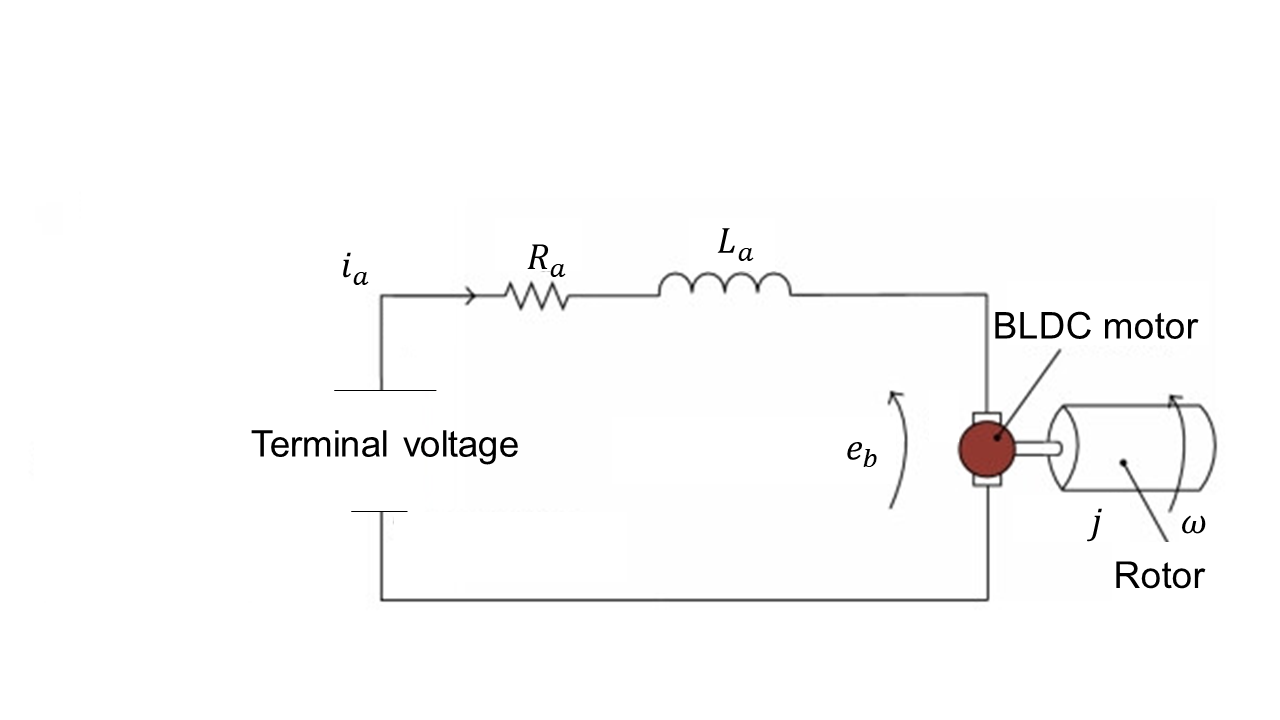
\includegraphics[width=0.5\linewidth]{figures/per phase circuit of BLDC.png}

    \caption{Per phase equivalent circuit of a trapezoidal BLDC motor } %\cite{xiang2015practical}
    %\caption*{Source: \cite{xiang2015practical}}

    \label{fig:BLDC MOTOR}
\end{figure}

%The motor torque is proportional to the armature current,

%\begin{equation*}
%\tau_m = K_\tau i_a
%\end{equation*}

%thus

%\begin{equation*}
%i_a = \frac{\tau_m}{K_\tau}
%\end{equation*}

%The electrical power consumed at hovering is

%\begin{equation*}
%P = V_a i_a = K_v \Omega \frac{\tau_m}{K_\tau}
%\end{equation*}

%Assuming the motor torque is proportional to the generated thrust, i.e., 
%$\tau_m = K_t T$, the power becomes

%\begin{equation}
%P = \frac{K_v}{K_\tau} K_t T \Omega
%\label{3.19}
%\end{equation}

%Combining equation~\eqref{3.18} with equation~\eqref{3.19} yields

%\begin{equation*}
%\frac{T^{\tfrac{3}{2}}}{\sqrt{\rho A}} = \frac{K_v}{K_\tau} K_t T \Omega
%\end{equation*}

%which simplifies to

%\begin{equation*}
%T^{\tfrac{1}{2}} = \frac{K_v}{K_\tau} K_t \sqrt{\rho A} \, \Omega
%\end{equation*}

%Squaring both sides gives

%\begin{equation*}
%T = \left[ \frac{K_v}{K_\tau} K_t \sqrt{\rho A} \right]^2 \Omega^2
%\end{equation*}

%Let

%\[
%b = \left[ \frac{K_v}{K_\tau} K_t \sqrt{\rho A} \right]^2
%\]

%where $b$ denotes the thrust coefficient. Hence,

%\begin{equation}
%T = b \Omega^2
%\label{3.20}
%\end{equation}


%%%%%%%%%%%%%%%%%%%%%%%%%%%
The actuator dynamics of the propeller motor assembly can be derived from the electrical and electromechanical relationships of the trapezoidal BLDC motor. Since the voltage equation of a trapezoidal BLDC motor is similar to that of a conventional DC motor, Kirchhoff’s Voltage Law (KVL) applied to the per phase equivalent circuit shown in Figure~\ref{fig:BLDC MOTOR} gives
\begin{equation}
V_a = R_a i_a + L_a \frac{di_a}{dt} + e_b
\end{equation}
where $V_a$ is the applied terminal voltage (V), $R_a$ is the stator phase resistance ($\Omega$), $L_a$ is the stator phase inductance (H), $i_a$ is the stator current (A), and $e_b$ is the back electromotive force (V).

The back electromotive force is proportional to the rotor angular velocity and is expressed as
\begin{equation}
e_b = K_v \Omega
\end{equation}
where $K_v$ is the back electromotive force (EMF)  constant (V\,s/rad) and $\Omega$ is the rotor angular velocity (rad/s).

Under steady state operation and for a simplified actuator model, the voltage drops across the stator resistance and inductance are assumed negligible compared to the back-EMF. Therefore, the voltage equation reduces to
\begin{equation}
V_a \approx e_b = K_v \Omega
\end{equation}

The electromagnetic torque produced by the motor is proportional to the stator current, that is,
\begin{equation}
\tau_m = K_{\tau} i_a
\end{equation}
where $\tau_m$ is the motor electromagnetic torque (N\,m) and $K_{\tau}$ is the motor torque constant (N\,m/A). Rearranging gives
\begin{equation}
i_a = \frac{\tau_m}{K_{\tau}}
\end{equation}

The electrical power consumed by the motor during hovering is given by
\begin{equation}
P = V_a i_a
\end{equation}
where $P$ is the electrical input power (W). Substituting $V_a = K_v \Omega$ and $i_a = \tau_m / K_{\tau}$ yields
\begin{equation}
P = K_v \Omega \frac{\tau_m}{K_{\tau}}
\end{equation}

For the propeller motor system, the motor torque is assumed proportional to the generated thrust. Thus,
\begin{equation}
\tau_m = K_t T
\end{equation}
where $K_t$ is the torque thrust proportionality constant and $T$ is the thrust generated by the propeller (N). Substituting this relation into the power expression gives
\begin{equation}
P = \frac{K_v}{K_{\tau}} K_t T \Omega
\label{eq:motor_power}
\end{equation}

On the other hand, from momentum theory, the aerodynamic power required to generate thrust can be expressed as
\begin{equation}
P = \frac{T^{3/2}}{\sqrt{\rho A}}
\label{eq:aero_power}
\end{equation}
where $\rho$ is the air density (kg/m$^3$) and $A$ is the rotor disc area (m$^2$).

Combining \eqref{eq:aero_power} and \eqref{eq:motor_power} gives
\begin{equation}
\frac{T^{3/2}}{\sqrt{\rho A}} = \frac{K_v}{K_{\tau}} K_t T \Omega
\end{equation}

Dividing both sides by $T$ results in
\begin{equation}
T^{1/2} = \frac{K_v}{K_{\tau}} K_t \sqrt{\rho A}\,\Omega
\end{equation}

Squaring both sides gives
\begin{equation}
T = \left( \frac{K_v}{K_{\tau}} K_t \sqrt{\rho A} \right)^2 \Omega^2
\end{equation}

Let
\begin{equation}
b = \left( \frac{K_v}{K_{\tau}} K_t \sqrt{\rho A} \right)^2
\end{equation}
where $b$ denotes the lumped thrust coefficient. Hence, the thrust generated by the propeller is obtained as
\begin{equation}
T = b \Omega^2
\label{3.20}
\end{equation}

Equations~\eqref{eq:motor_power}--\eqref{3.20} show that the thrust produced by the BLDC motor--propeller actuator is proportional to the square of the rotor angular velocity. This relationship is commonly used in quadrotor dynamic modeling and control design.


%%%%%%%%%%%%%%%%%%%%%%%%

Equation~\eqref{3.20} shows that the thrust produced by each propeller is proportional 
to the square of its angular speed. Using equations~\eqref{3.18} and~\eqref{3.20}, the 
relationship among propeller speed, thrust, and power can be determined. Consequently, 
the required power delivered by the Electronic Speed Controller (ESC) to the BLDC motor 
can be estimated in order to achieve the desired propeller speed and generate the thrust 
necessary to drive the quadrotor according to the commanded input.




%%%%%%%%%%%%%%%%%%%%%



\subsubsubsection{\textbf{Total Thrust Force and Moments Derivation}}

Based on free body diagram of Quadrotor in Figure\ref{fig:Quadrotor free body diagram} and equation \eqref{3.20}, 
\textbf{total thrust force} $U_1$ due to rotation of each propeller is solved as follows: 
Since all the thrust forces are acting in upward direction:

\begin{equation}
U_1 = T_1 + T_2 + T_3 + T_4 = b\Omega_1^2 + b\Omega_2^2 + b\Omega_3^2 + b\Omega_4^2 = b(\Omega_1^2 + \Omega_2^2 + \Omega_3^2 + \Omega_4^2)
\label{3.21}
\end{equation}
%\end{equation*}

%\begin{equation}
%U_1 = b(\Omega_1^2 + \Omega_2^2 + \Omega_3^2 + \Omega_4^2)
%\tag{3.21}
%\label{3.21}
%\end{equation}

The \textbf{rolling control torque} $U_2$ in positive $\phi$ direction is solved as follows:

\begin{equation}
U_2 = \ell (T_1 - T_2 - T_3 + T_4) 
    = \ell (b\Omega_1^2 - b\Omega_2^2 - b\Omega_3^2 + b\Omega_4^2)  = \ell b(\Omega_1^2 - \Omega_2^2 - \Omega_3^2 + \Omega_4^2)
    \label{3.22}
\end{equation}


Where $\ell$ is distance between rotor center and CoG of Quadrotor, and the positive and 
negative sign indicate the rotor at which their speed increase and decrease, respectively, 
in the way that maintaining the overall thrust $U_1$ constant.

%\begin{equation}
%U_2 = \ell b(\Omega_1^2 - \Omega_2^2 - \Omega_3^2 + \Omega_4^2)
%\tag{3.22}
%\label{3.22}
%\end{equation}

The \textbf{pitching control torque} $U_3$ in positive $\theta$ direction is solved as follows:

\begin{equation}
U_3 = \ell (T_1 + T_2 - T_3 - T_4) 
    = \ell (b\Omega_1^2 + b\Omega_2^2 - b\Omega_3^2 - b\Omega_4^2) = \ell b(\Omega_1^2 + \Omega_2^2 - \Omega_3^2 - \Omega_4^2)
%\tag{3.23}
\label{3.23}
\end{equation}

%\begin{equation}
%U_3 = \ell b(\Omega_1^2 + \Omega_2^2 - \Omega_3^2 - \Omega_4^2)
%\tag{3.23}
%\label{3.23}
%\end{equation}


The \textbf{yaw control torque} $U_4$ is solved based on the concept of Newton third law of motion, 
which states that for any action torque there is reactive torque generated by drag torque $\tau_i (i=1,2,3,4)$. 
Due to this drag torque, yaw rotation is caused in the direction of net drag torque. 
For instance, if $(\tau_2 + \tau_4) > (\tau_1 + \tau_3)$, the Quad will rotate in positive yaw direction. 
In the same way as equation \eqref{3.20}, drag torque mathematically formulated as $\tau = d\Omega^2$, 
where $d$ is aerodynamic drag coefficient. Hence, yaw control torque becomes:

\begin{equation}
U_4 = d(-\Omega_1^2 + \Omega_2^2 - \Omega_3^2 + \Omega_4^2)
%\tag{3.24}
\label{3.24}
\end{equation}

By combining equations \eqref{3.21}-\eqref{3.24}, control mixing matrix is derived as follows:

\begin{equation}
\begin{bmatrix}
U_1 \\[6pt]
U_2 \\[6pt]
U_3 \\[6pt]
U_4
\end{bmatrix}
=
\begin{bmatrix}
b   & b   & b   & b   \\[6pt]
b\ell & -b\ell & -b\ell & b\ell \\[6pt]
b\ell & b\ell & -b\ell & -b\ell \\[6pt]
-d  & d   & -d  & d
\end{bmatrix}
\begin{bmatrix}
\Omega_1^2 \\[6pt]
\Omega_2^2 \\[6pt]
\Omega_3^2 \\[6pt]
\Omega_4^2
\end{bmatrix}    
\end{equation}

%\]


By using \textbf{Symbolic Math Toolbox}$^{\text{TM4}}$ in MATLAB$^{\text{\textregistered}}$, 
Then, \textbf{Control allocation or mixing} equations become:

%\[
%\begin{bmatrix}
%\Omega_1^2 \\[8pt]
%\Omega_2^2 \\[8pt]
%\Omega_3^2 \\[8pt]
%\Omega_4^2
%\end{bmatrix}
%=
%\begin{bmatrix}
%\dfrac{1}{4b} & \dfrac{1}{4b\ell} & \dfrac{1}{4b\ell} & -\dfrac{1}{4d} \\[12pt]
%\dfrac{1}{4b} & -\dfrac{1}{4b\ell} & \dfrac{1}{4b\ell} & \dfrac{1}{4d} \\[12pt]
%\dfrac{1}{4b} & -\dfrac{1}{4b\ell} & -\dfrac{1}{4b\ell} & -\dfrac{1}{4d} \\[12pt]
%\dfrac{1}{4b} & \dfrac{1}{4b\ell} & -\dfrac{1}{4b\ell} & \dfrac{1}{4d}
%\end{bmatrix}
%\begin{bmatrix}
%U_1 \\[8pt]
%U_2 \\[8pt]
%U_3 \\[8pt]
%U_4
%\end{bmatrix}
%\]


%Then, \textbf{Control allocation or mixing} equations become:

%\begin{subequations}
 % \renewcommand\theequation{3.30\alph{equation}} % -> (3.30a–d)
 % \begin{empheq}[left=\empheqlbrace]{align}
   % \Omega_1 &= \sqrt{\tfrac{U_1}{4b} + \tfrac{U_2}{4b\ell} + \tfrac{U_3}{4b\ell} - \tfrac{U_4}{4d}} \label{eq:330a}\\[8pt]
   % \Omega_2 &= \sqrt{\tfrac{U_1}{4b} - \tfrac{U_2}{4b\ell} + \tfrac{U_3}{4b\ell} + \tfrac{U_4}{4d}} \label{eq:330b}\\[8pt]
    %\Omega_3 &= \sqrt{\tfrac{U_1}{4b} - \tfrac{U_2}{4b\ell} - \tfrac{U_3}{4b\ell} - \tfrac{U_4}{4d}} \label{eq:330c}\\[8pt]
    %\Omega_4 &= \sqrt{\tfrac{U_1}{4b} + \tfrac{U_2}{4b\ell} - \tfrac{U_3}{4b\ell} + \tfrac{U_4}{4d}} \label{eq:330d}
  %\end{empheq}
%\end{subequations}

\begin{equation}
\left\{
\begin{aligned}
 \Omega_1 &= \sqrt{\tfrac{U_1}{4b} + \tfrac{U_2}{4b\ell} + \tfrac{U_3}{4b\ell} - \tfrac{U_4}{4d}} \\[8pt]
    \Omega_2 &= \sqrt{\tfrac{U_1}{4b} - \tfrac{U_2}{4b\ell} + \tfrac{U_3}{4b\ell} + \tfrac{U_4}{4d}} \\[8pt]
    \Omega_3 &= \sqrt{\tfrac{U_1}{4b} - \tfrac{U_2}{4b\ell} - \tfrac{U_3}{4b\ell} - \tfrac{U_4}{4d}} \\[8pt]
    \Omega_4 &= \sqrt{\tfrac{U_1}{4b} + \tfrac{U_2}{4b\ell} - \tfrac{U_3}{4b\ell} + \tfrac{U_4}{4d}} 
\end{aligned}
\right.
%\tag{3.25}
\label{3.25}
\end{equation}

%\subsubsection{The Overall Governing Equations of Quadrotor Dynamics}

By combining Newton-Quaternion approach which described in equations \eqref{3.9} - \eqref{3.25} we have 
\begin{equation}
\left\{
\begin{aligned}
 \ddot{x} &= 2(q_1q_3 - q_0q_2)\tfrac{U_1}{m} - \tfrac{C_{dx}}{m}\dot{x} \\[-3pt]
\ddot{y} &= 2(q_2q_3 + q_0q_1)\tfrac{U_1}{m} - \tfrac{C_{dy}}{m}\dot{y} \\[-3pt]
\ddot{z} &= \big[2(q_0^2+q_3^2)-1\big]\tfrac{U_1}{m} - g - \tfrac{C_{dz}}{m}\dot{z} \\[-3pt]
\dot{p} &= \tfrac{1}{J_{xx}}U_2+\tfrac{J_{yy}-J_{zz}}{J_{xx}}qr-\tfrac{J_p}{J_{xx}}q\Omega_r-\tfrac{C_{a_p}}{J_{xx}}p \\[-3pt]
\dot{q} &= \tfrac{1}{J_{yy}}U_3+\tfrac{J_{zz}-J_{xx}}{J_{yy}}pr+\tfrac{J_p}{J_{yy}}p\Omega_r-\tfrac{C_{a_q}}{J_{yy}}q \\[-3pt]
\dot{r} &= \tfrac{1}{J_{zz}}U_4+\tfrac{J_{xx}-J_{yy}}{J_{zz}}pq-\tfrac{C_{a_r}}{J_{zz}}r \\[-3pt]
\dot{q}_0 &= -\tfrac{1}{2}(pq_1+qq_2+rq_3) \\[-3pt]
\dot{q}_1 &= \tfrac{1}{2}(pq_0+rq_2-qq_3) \\[-3pt]
\dot{q}_2 &= \tfrac{1}{2}(qq_0+pq_3-rq_1) \\[-3pt]
\dot{q}_3 &= \tfrac{1}{2}(rq_0+qq_1-pq_2) 
\end{aligned}
\right.
%\tag{3.26}
\label{3.26}
\end{equation}
%%%%%%%%%%%%%%%%%%%%

From the quadrotor governing dynamics in equation~\eqref{3.26}, the system can be interpreted 
as a \textit{cascade structure}. The translational dynamics depend on the attitude states of 
the rotational dynamics, whereas the rotational dynamics are independent of the translational 
states. This property will later be exploited in controller design. 

The \textbf{control mixing (or control allocation) equations} take the control inputs and 
transform them into the corresponding rotor angular speeds. The overall residual (net) 
propeller angular speed is given by

\begin{equation}
\Omega_r = -\Omega_1 + \Omega_2 - \Omega_3 + \Omega_4
\label{3.27}
\end{equation}

The quaternion-based quadrotor dynamics in equation~\eqref{3.26} involve simple quaternion 
operations, which reduce computational cost and improve numerical stability. In addition, 
quaternion representation enables the design of singularity-free controllers capable of 
operating at all attitudes, thereby allowing agile flight and aerobatic maneuvers~\cite{nekoo2022quaternion}. 
However, quaternions are less intuitive for visualization and interpretation.

To address this limitation, quaternion states are often converted into Euler angles, which 
are easier to interpret. Using the canonical Euler set, roll and yaw lie within $[-\pi,\pi]$ 
while pitch lies within $\left[-\tfrac{\pi}{2},\,\tfrac{\pi}{2}\right]$. The relationship 
between quaternion and Euler angles is expressed as~\cite{schreier2013quaternion}

\begin{equation}
\begin{bmatrix}
\phi \\[4pt]
\theta \\[4pt]
\psi
\end{bmatrix}
=
\begin{bmatrix}
\arctan 2\big(2(q_0q_1+q_2q_3),\, q_0^2 - q_1^2 - q_2^2 + q_3^2\big) \\[6pt]
\arcsin\big(2(q_0q_2 - q_3q_1)\big) \\[6pt]
\arctan 2\big(2(q_0q_3+q_1q_2),\, q_0^2+q_1^2-q_2^2-q_3^2\big)
\end{bmatrix}
\label{3.28}
\end{equation}

Thus, the quaternion formulation in equation~\eqref{3.26} avoids the singularity problem 
encountered in Euler representation (e.g., when the pitch angle approaches 
$\tfrac{\pi}{2}$ rad), while the conversion in equation~\eqref{3.28} allows convenient 
visualization and interpretation of the quadrotor orientation.


%%%%%%%%%%%%%%%%%%




%\chapter{CONTROLLER DESIGN}

\section{Design of Controller for Quadcopter}

%Despite having four rotors, the translational dynamics of quadcopters tend to be underactuated. This indicates that they are not equipped with enough control inputs to directly regulate every degree of freedom (DOF), particularly lateral motion. The system is enhanced by incorporating virtual control inputs, aiming to ensure that each output of the quadrotor aligns with a predetermined trajectory \cite{li2018model}. The following can be used to obtain the virtual control inputs:

Despite the presence of four rotors, the translational dynamics of a quadcopter remain underactuated. 
This means that the system does not possess a sufficient number of independent control inputs to 
directly regulate all degrees of freedom (DOF), especially the lateral motions. To overcome this 
limitation, virtual control inputs are introduced so that each output of the quadrotor can follow a 
predefined reference trajectory \cite{li2018model}. The virtual control inputs can be obtained as follows:


\begin{equation}
\begin{cases}
U_x = 2(q_{1}q_{3} - q_{0}q_{2})\,U_{1} - C_{dx}\dot{x}, \\[8pt]
U_y = 2(q_{2}q_{3} + q_{0}q_{1})\,U_{1} - C_{dy}\dot{y}, \\[8pt]
U_z = \Big[2(q_{0}^{2} + q_{3}^{2}) - 1\Big]U_{1} - m g - C_{dz}\dot{z}.
\end{cases}
%\tag{18}
\label{eq:virtual control inputs}
\end{equation}




%\begin{equation}
%U_x = 2(q_{1}q_{3} - q_{0}q_{2})U_{1} - C_{dx}\dot{x},
%\end{equation}

%\begin{equation}
%U_y = 2(q_{2}q_{3} + q_{0}q_{1})U_{1} - C_{dy}\dot{y},
%\end{equation}

%\begin{equation}
%U_z = \big[2(q_{0}^{2} + q_{3}^{2}) - 1\big]U_{1} - mg - C_{dz}\dot{z}.
%\label{virtual control inputs}
%\end{equation}

%where the parameters $U_x$, $U_y$, and $U_z$ denote the virtual control inputs for guiding the quadrotor position along the $x$, $y$, and $z$ axes respectively. The quadrotor translational dynamics can be represented as: \eqref{eq:virtual control inputs}

Here, the parameters $U_x$, $U_y$, and $U_z$ represent the virtual control inputs responsible 
for directing the quadrotor’s position along the $x$-, $y$-, and $z$-axes, respectively. 
Accordingly, the translational dynamics of the quadrotor can be expressed as shown in 
\eqref{eq:virtual control inputs}.


\begin{equation}
\ddot{x} = \frac{U_x}{m}, \quad 
\ddot{y} = \frac{U_y}{m}, \quad 
\ddot{z} = \frac{U_z}{m}.
\label{eq:simplified translation dynamics}
\end{equation}


To design controller for a second order system, the rotational dynamics of a quadrotor are 
rewritten in quaternion using the small quaternion approach.

\begin{equation}
\begin{bmatrix}
\dot{q}_0 \\ \dot{q}_1 \\ \dot{q}_2 \\ \dot{q}_3
\end{bmatrix}
= \tfrac{1}{2}
\begin{bmatrix}
1 & 0 & 0 & 0 \\
0 & 1 & 0 & 0 \\
0 & 0 & 1 & 0 \\
0 & 0 & 0 & 1
\end{bmatrix}
\begin{bmatrix}
0 \\ p \\ q \\ r
\end{bmatrix}
= \tfrac{1}{2}
\begin{bmatrix}
0 \\ p \\ q \\ r
\end{bmatrix} 
\end{equation}



Hence, making angular velocity the subject and differentiating we have.

\begin{equation}
\begin{bmatrix}
p \\ q \\ r
\end{bmatrix}
= 2
\begin{bmatrix}
\dot{q}_1 \\ \dot{q}_2 \\ \dot{q}_3
\end{bmatrix}, \begin{bmatrix}
\dot{p} \\ \dot{q} \\ \dot{r}
\end{bmatrix}
= 2
\begin{bmatrix}
\ddot{q}_1 \\ \ddot{q}_2 \\ \ddot{q}_3
\end{bmatrix}
\end{equation}

%\[
%\begin{bmatrix}
%\dot{p} \\ \dot{q} \\ \dot{r}
%\end{bmatrix}
%= 2
%\begin{bmatrix}
%\ddot{q}_1 \\ \ddot{q}_2 \\ \ddot{q}_3
%\end{bmatrix}
%\]

Finally, the second-order rotational dynamics of the quadrotor can be expressed using quaternions as follows:


\begin{equation}
\left\{
\begin{aligned}
\ddot{q}_{1} &= \frac{1}{J_{xx}} U_{2} 
+ \frac{J_{yy} - J_{zz}}{J_{xx}} qr 
- \frac{J_{p}}{J_{xx}} q \Omega_{r} 
- \frac{C_{ap}}{J_{xx}} p, \\[8pt]
\ddot{q}_{2} &= \frac{1}{J_{yy}} U_{3} 
+ \frac{J_{zz} - J_{xx}}{J_{yy}} pr 
+ \frac{J_{p}}{J_{yy}} p \Omega_{r} 
- \frac{C_{aq}}{J_{yy}} q, \\[8pt]
\ddot{q}_{3} &= \frac{1}{J_{zz}} U_{4} 
+ \frac{J_{xx} - J_{yy}}{J_{zz}} pq 
- \frac{C_{ar}}{J_{zz}} r.
\end{aligned}
\right.
%\tag{23}
\label{eq:second-order rotational dynamics}
\end{equation}



The state vector is composed of two components: orientation control, expressed as 
$[q_{1}, \dot{q}_{1}, q_{2}, \dot{q}_{2}, q_{3}, \dot{q}_{3}]$ 
and position control, expressed as 
$[x, \dot{x}, y, \dot{y}, z, \dot{z}]$.


\subsection{Design of a quadrotor position controller}

%The first step to design an improved nonsingular adaptive super twisting sliding mode controller is designing sliding manifold of SMC. SMC enables the design of controllers for both linear and nonlinear processes. The concept of the SMC technique is to force the command signal to move to the sliding surface and stay on that surface after the command signal has been reached. In order to guarantee that the system states stay on the sliding surface, the control law is then designed. The two phases of SMC are \cite{iqbal2019modern}:

%\textbf{Reaching phase:} This phase involves designing the control law to drive the system’s state trajectories towards a predefined sliding surface. The sliding surface is a manifold where the control objectives are met. During the reaching phase, a discontinuous control law is applied to force the system to reach the sliding surface despite the presence of uncertainties and disturbances.  

%\textbf{Sliding phase:} Once the system state reaches the sliding surface, the control switches to ensure that the state remains on this surface for all times. This phase is characterized by the system’s dynamics being confined to the sliding surface, designed to be invariant. The control law in this phase maintain the system on the sliding surface, ensuring robust performance against perturbations and uncertainties.  

%These phases are crucial for ensuring that SMC achieves its robustness and performance 
%despite the presence of uncertainties and external disturbances.Figure\ref{fig:Controller architecture for quadrotor}, illustrates the complete controller architecture, including the position and altitude controllers, as well as the virtual control input.  

\begin{figure}[h!]
    \centering
    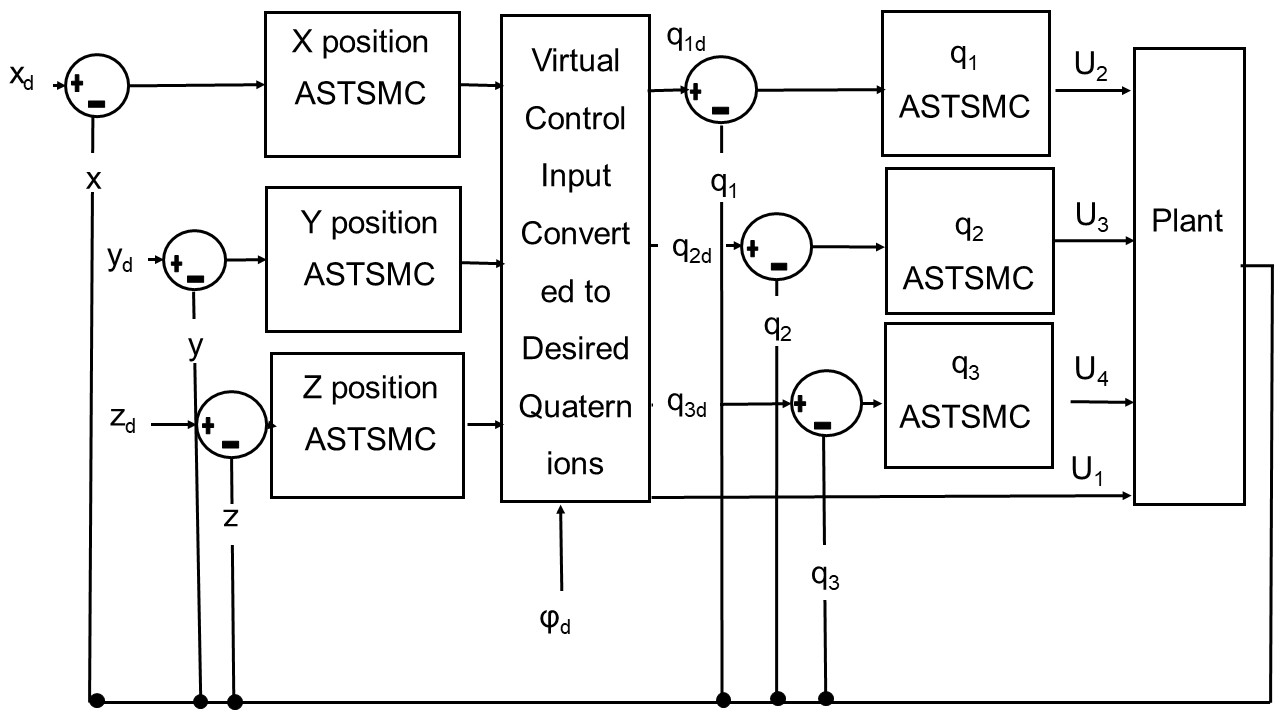
\includegraphics[width=0.65\linewidth]{figures/Fig2.General architecture for UAV quadcopter control.jpg}
    \caption{Controller architecture for quadrotor, including position, altitude, and virtual control input designs}
    %\caption{Controller architecture for quadrotor, including position, altitude, and virtual control input designs\cite{abera2024improved}}
    \label{fig:Controller architecture for quadrotor}
\end{figure}





%\textbf{Design sliding manifold.} The following procedures should be taken to design a sliding manifold.  
  Figure\ref{fig:Controller architecture for quadrotor} shows the general architecture for both position and attitude controller, in this figure desired $x_d,y_d $ and $z_d$ are compared with actual $x,y $ and $z$ then the errors are fed to sliding surface and then a position control law are implemented and results to virtual control inputs which are then combined with desired yaw angle and converted to desired quaternions which then be used as reference to actual quaternion ready for manipulating and obtain roll,pitch and yaw control inputs. It is proposed that firstly a position controller be designed using following steps.
\begin{enumerate}
  \item Determine the quadcopter desired trajectory.
  \begin{equation}
  \begin{bmatrix}
  e_x \\ e_y \\ e_z
  \end{bmatrix}
  =
  \begin{bmatrix}
  x_d - x \\ y_d - y \\ z_d - z
  \end{bmatrix},
  \quad
  \begin{bmatrix}
  \dot{e}_x \\ \dot{e}_y \\ \dot{e}_z
  \end{bmatrix}
  =
  \begin{bmatrix}
  \dot{x}_d - \dot{x} \\ \dot{y}_d - \dot{y} \\ \dot{z}_d - \dot{z}
  \end{bmatrix}
  \label{eqn:surface errors}
  %\tag{4.6}
  \end{equation}

  %\item Design a sliding manifold, a function that measures the difference between the quadcopter actual and desired states. Designing the sliding surface in accordance with the dynamics of the error is the first stage in minimizing the difference between the desired and the actual value, and Stoline and Li proposed the general form of the following equation in~\cite{bouabdallah2004pid}:

  \item Design sliding surfaces
  
 % \begin{equation}
%\sigma = \left( \lambda + \frac{d}{dt} \right)^p e
%\label{eq:sliding_general}
%\tag{4.7}
%\end{equation}


%where $e$ is the tracking error, defined as for z-axis $e(z) = z_d - z$ (the error between the desired trajectory and the actual trajectory in the x-axis); $\lambda$ and $c$ is a positive constant that interprets the dynamics of the surface and $p=n-1$, $n$ is relative degree between output and input. Based on Eq.~\eqref{eq:sliding_general}, position controller sliding manifold can be designed:

\begin{equation}
\begin{cases}
\sigma_x = \lambda_x e_x + c_x \dot{e}_x, \\
\sigma_y = \lambda_y e_y + c_y \dot{e}_y, \\
\sigma_z = \lambda_z e_z + c_z \dot{e}_z
\label{eq:position sliding manifold}
\end{cases}
%\tag{4.8}
\end{equation}
Where  $ \lambda_i $  and   $c_i$  denotes positive position error and velocity error respectively.

\noindent
3. Design control law and tune the gain of sliding surface using PSO.

\subsection*{Design super twisting sliding mode controller}
STSMC is given by the equation below:

\begin{equation}
U_{st} = -\alpha \sqrt{|\sigma|}\,\text{sign}(\sigma) - \nu
\label{eq:supertwisting for x axis}
%\tag{4.9}
\end{equation}

\begin{equation}
\dot{\nu} = \frac{\beta}{2}\,\text{sign}(\sigma)
\label{eq:v_x}
%\tag{4.10}
\end{equation}

The total control law ($U$) calculated by summing the equivalent and supertwisting control law:

\begin{equation}
U = U_{equ} + U_{st}
\label{eq:total control law}
%\tag{4.11}
\end{equation}

where $U_{equ}$ is equivalent controller and $U_{st}$ is super twisting controller. 

Fig.~\ref{fig:position controller smc} illustrates the position controller diagram designed for the quadcopter. The controller focuses on maintaining the desired trajectory by controlling the quadcopter position in the $x$, $y$, and $z$ axes.

After selecting the sliding surface, the next step is to design the equivalent control law, and this law ensures the system remains in sliding mode during operation. Equivalent control law can be designed by making $\dot{\sigma}_x, \dot{\sigma}_y, \dot{\sigma}_z = 0$.

The virtual controller $(U_x, U_y, U_z)$ which means that the three common input will control
motion along x, y and z and these virtual control are given by equation.
\begin{equation}
\left\{
\begin{aligned}
U_x &= \frac{\lambda_x}{c_x}\dot{e}_x + \ddot{x}_d - \alpha_x \sqrt{|\sigma_x|}\, \text{sign}(\sigma_x) - v_x, \\[6pt]
U_y &= \frac{\lambda_y}{c_y}\dot{e}_y + \ddot{y}_d - \alpha_y \sqrt{|\sigma_y|}\, \text{sign}(\sigma_y) - v_y, \\[6pt]
U_z &= \frac{\lambda_z}{c_z}\dot{e}_z + \ddot{z}_d - \alpha_z \sqrt{|\sigma_z|}\, \text{sign}(\sigma_z) - v_z.
\end{aligned}
\right.
\label{eq:virtual control law for position}
%\tag{4.12}
\end{equation}

where $\alpha, \beta$ are the gain of super twisting algorithm and 
$\dot{v} = -\frac{\beta}{2}\text{sign}(\sigma)$.




%\begin{figure}[h!]
   % \centering
   % 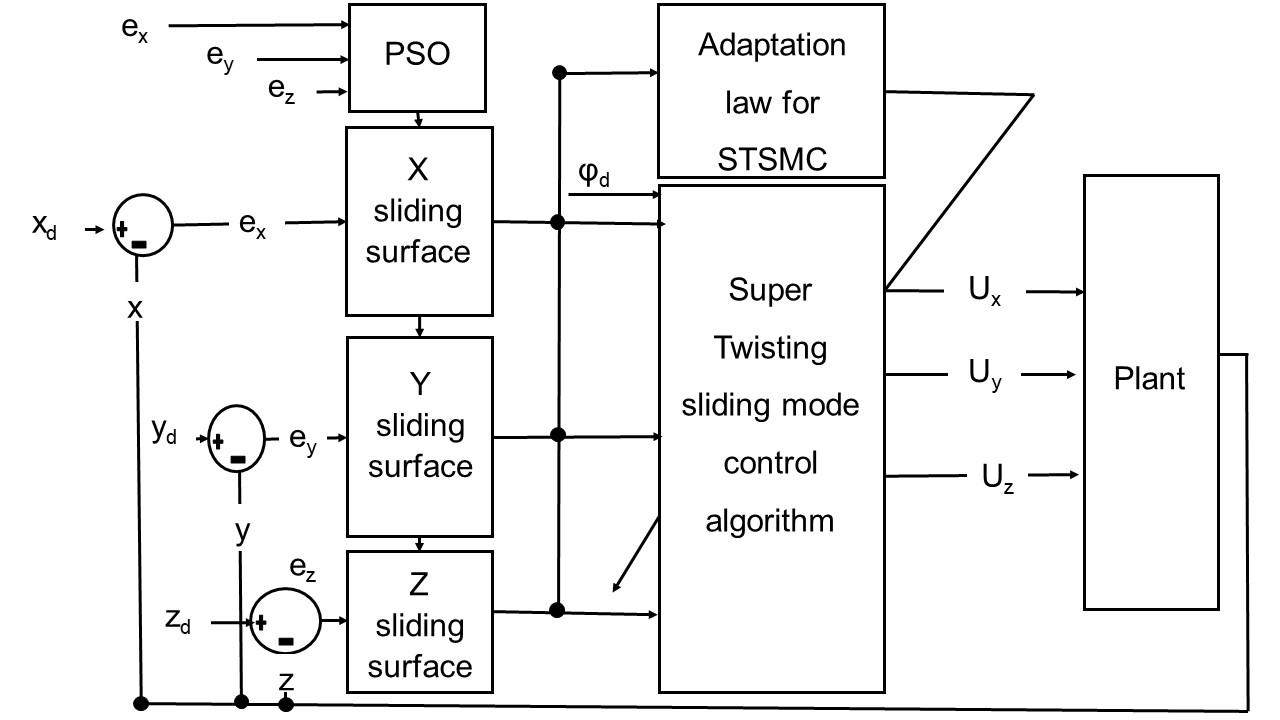
\includegraphics[width=1.0\linewidth]{figures/Fig3.Position Controller for UAV quadcopter - Copy.jpg}
    %\caption{Diagram of position controller for maintaining quadrotor trajectory along x,y,and zaxes}
    %\caption{Diagram of position controller for maintaining quadrotor trajectory along x,y,and zaxes\cite{abera2024improved}}
   % \label{fig:position controller smc}
%\end{figure}

\begin{figure}[h!]
    \centering
    \begin{minipage}{0.48\linewidth}
        \centering
        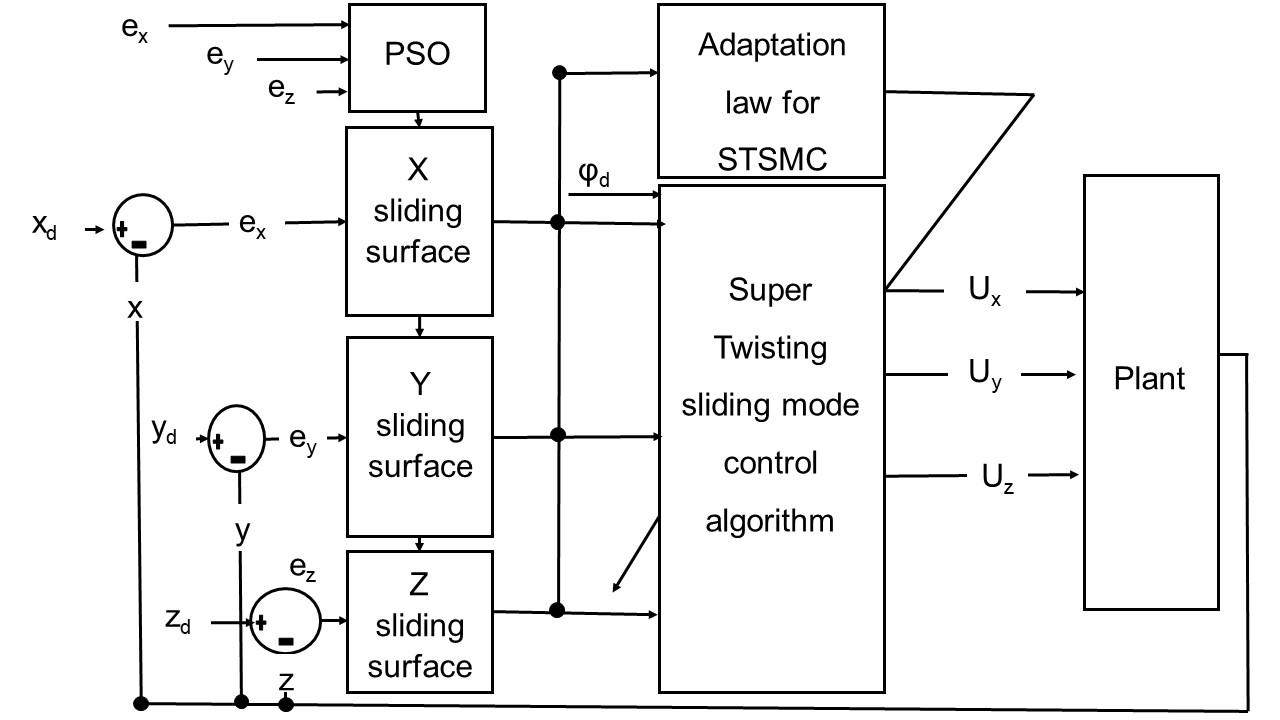
\includegraphics[width=1.0\linewidth]{figures/Fig3.Position Controller for UAV quadcopter - Copy.jpg}
        \caption{Diagram of position controller for maintaining quadrotor trajectory along x,y,and zaxes}
        \label{fig:position controller smc}
    \end{minipage}
    \hfill
    \begin{minipage}{0.48\linewidth}
        \centering
       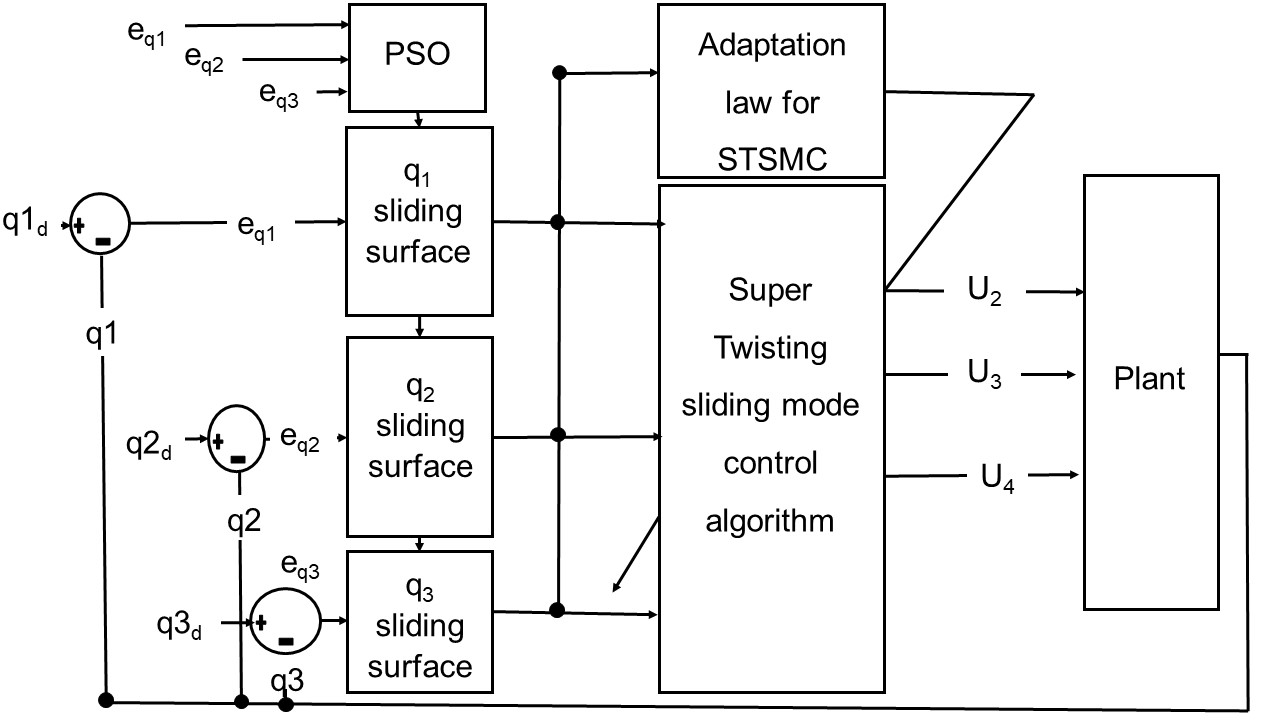
\includegraphics[width=1\linewidth]{figures/Fig4.Attitude Controller for UAV quadcopter.jpg}
    \caption{Altitude controller diagram for maintaining desired quadrotor altitude}
   % \caption{Altitude controller diagram for maintaining desired quadrotor altitude\cite{abera2024improved}}
    \label{fig:attitude controller}
    \end{minipage}
\end{figure}




\begin{theorem}
If the quadrotor position system~\eqref{3.26}, is taken into consideration, together with the
PSO based sliding manifold~\eqref{eq:supertwisting for x axis}, control laws~\eqref{eq:virtual control law for position}, and tracking errors~\eqref{eqn:surface errors}, 
asymptotically, the closed loop tracking error can approach zero. 

The control law must ensure that $\dot{V}(z) < 0$ and the system state variables $V(z) > 0$.
\end{theorem}

\noindent \textbf{Proof.} 
Lyapunov function is a positive scalar function, defined as
\begin{equation}
    V_z = \tfrac{1}{2} \sigma^T \sigma = \tfrac{1}{2} \sigma^2 \sigma.
\end{equation}


Now differentiating $V_z$ with respect to time it was found to be:

%The control law must ensure that $\dot{V}(z) < 0$ and the system state variables $V(z) > 0$.
\begin{equation}
\begin{align*}
\dot{V}_z &= \sigma_z \dot{\sigma}_z < 0  = \sigma_z \big(\lambda_z \dot{e}_z + c_z (\ddot{z}_d - \ddot{z})\big)\\[6pt]
%\dot{V}_z &= \sigma_z \big(\lambda_z \dot{e}_z + c_z (\ddot{z}_d - \ddot{z})\big)
\end{align*}  
\end{equation}


To substitute the value of $\ddot{z}$, use the virtual control law.
\begin{equation}
\begin{align*}
&= \lambda_z \dot{e}_z + c_z \Big(\ddot{z}_d - \alpha_z \sqrt{|\sigma_z|}\,\text{sign}(\sigma_z) 
   - \int \beta_z \,\text{sign}(\sigma_z)\, dt \Big)
\end{align*}
\end{equation}

\begin{equation}
\begin{align}
\dot{V}_z &= \sigma_z \Big(\lambda_z \dot{e}_z + c_z \ddot{z}_d - \lambda_z \dot{e}_z 
   - c_z \ddot{z}_d - \alpha_z \sqrt{|\sigma_z|}\,\text{sign}(\sigma_z) 
   - \int \beta_z \,\text{sign}(\sigma_z)\, dt \Big) \label{4.14} %\tag{4.13}
\end{align}
\end{equation}
\begin{equation}
\begin{align*}
\dot{V}_z &= \sigma_z \Big(-\alpha_z \sqrt{|\sigma_z|}\,\text{sign}(\sigma_z) 
   - \int \beta_z \,\text{sign}(\sigma_z)\, dt \Big) \leq 0
\end{align*}
\end{equation}
To make the Lyapunov function valid, the gains $\alpha_z, \beta_z$ should be above positive.


The virtual control in Eq.~\ref{eq:virtual control law for position}, used to determine desired quaternion value. 
When $x, y,$ and $z$ approach $x_d, y_d,$ and $z_d$ as time reaches the sliding surface 
$\sigma_x = 0, \; \sigma_y = 0, \; \sigma_z = 0$ and the designed controller derives the actual value 
to the desired position. The desired quaternion value can also be calculated by rearranging 
the virtual control inputs.


%\begin{subequations}
%\begin{align}
%U_1 &= \sqrt{U_x^2 + U_y^2 + (U_z + mg)^2} \tag{4.14} \\[8pt]
%q_{0d} &= \tfrac{1}{2}\sqrt{\frac{U_z + mg}{U_1} - 2\sin^2(\psi_d/2) + 1} \tag{4.15} \\[10pt]
%q_{1d} &= \sin(\psi_d/2)U_x + \tfrac{1}{\sqrt{2}}U_y
         % \sqrt{\frac{U_z + mg}{U_1} - 2\sin^2(\psi_d/2) + 1} \tag{4.16} \\[12pt]
%q_{2d} &= \frac{\sin(\psi_d/2)U_y - \tfrac{1}{\sqrt{2}}U_x
         % \sqrt{\frac{U_z + mg}{U_1} - 2\sin^2(\psi_d/2) + 1}}
         % {U_z + mg + U_1} \tag{4.17} \\[12pt]
%q_{3d} &= \sin\!\left(\tfrac{\psi_d}{2}\right) %\tag{4.18}
%\end{align}
%\end{subequations}

\begin{equation}
U_1 = \sqrt{U_x^2 + U_y^2 + (U_z + mg)^2}
%\tag{35}
\label{eq:35}
\end{equation}

\begin{equation}
\left\{
\begin{aligned}
q_{0d} &= \tfrac{1}{2} \sqrt{\frac{U_z + mg}{U_1} - 2\sin^2\!\left(\tfrac{\psi_d}{2}\right) + 1}, \\[8pt]
q_{1d} &= \sin\!\left(\tfrac{\psi_d}{2}\right) U_x 
+ \tfrac{1}{\sqrt{2}} U_y \sqrt{\frac{U_z + mg}{U_1} - 2\sin^2\!\left(\tfrac{\psi_d}{2}\right) + 1}, \\[8pt]
q_{2d} &= \frac{ \sin\!\left(\tfrac{\psi_d}{2}\right) U_y 
- \tfrac{1}{\sqrt{2}} U_x \sqrt{\frac{U_z + mg}{U_1} - 2\sin^2\!\left(\tfrac{\psi_d}{2}\right) + 1} }
{U_z + mg + U_1}, \\[8pt]
q_{3d} &= \sin\!\left(\tfrac{\psi_d}{2}\right).
\end{aligned}
\right.
%\tag{36}
\label{eq:36}
\end{equation}

\subsection{Attitude controller design}
\noindent
\textbf{Fig~\ref{fig:attitude controller}}, depicts the altitude controller diagram responsible for maintaining the quadcopter desired altitude. The controller operates by generating control input signals based on the reference inputs provided by the conversion blocks.
%\begin{figure}[h!]
  %  \centering
    %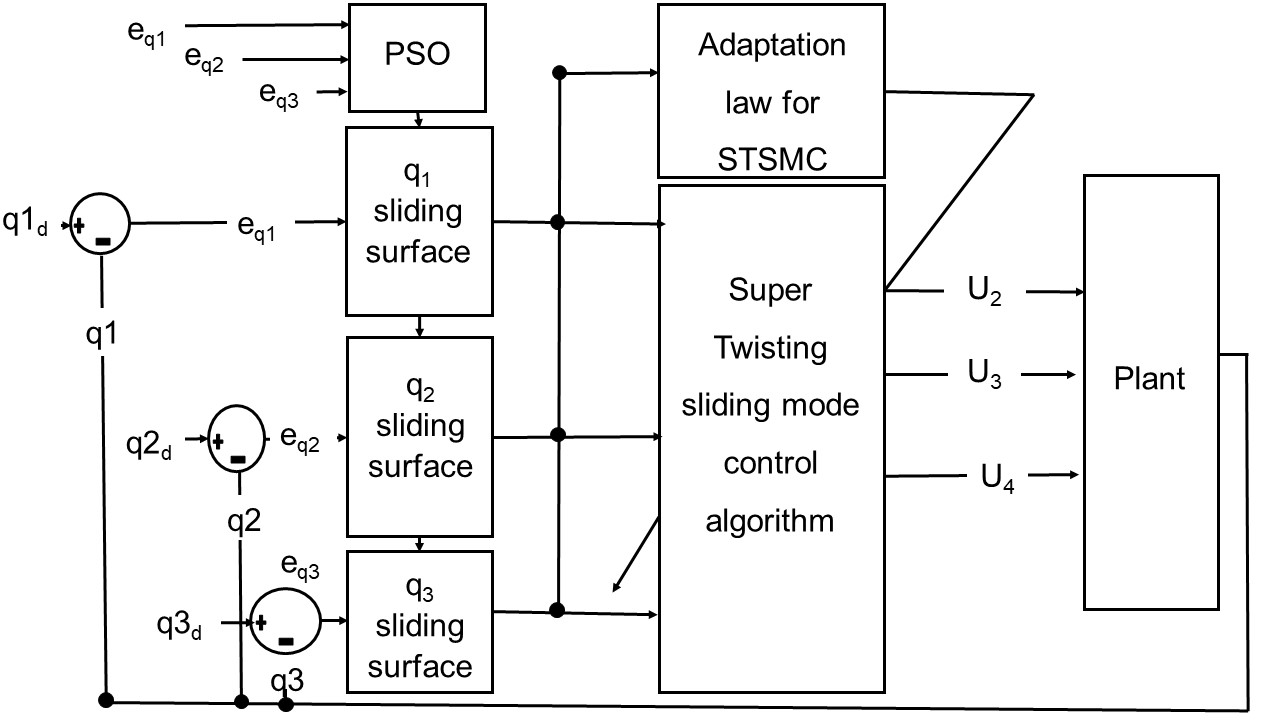
\includegraphics[width=1\linewidth]{figures/Fig4.Attitude Controller for UAV quadcopter.jpg}
   % \caption{Altitude controller diagram for maintaining desired quadrotor altitude}
   % \caption{Altitude controller diagram for maintaining desired quadrotor altitude\cite{abera2024improved}}
   % \label{fig:attitude controller}
%\end{figure}

By generating the input control signal $(U_2, U_3, U_4)$, the adaptive super twisting sliding 
mode control maintains the tracking errors of the attitude subsystem. 
The tracking errors are defined:
\begin{equation}
\begin{bmatrix}
e_{q_1} \\[6pt]
e_{q_2} \\[6pt]
e_{q_3}
\end{bmatrix}
=
\begin{bmatrix}
q_{1d} - q_1 \\[6pt]
q_{2d} - q_2 \\[6pt]
q_{3d} - q_3
\end{bmatrix}
\label{eq:attitude for error}
%\tag{4.20}
\end{equation}

Like position control design, to design altitude controller first step is designing of sliding surface:
\begin{equation}
\left\{
\begin{aligned}
\sigma_{q_1} &= \lambda_{q_1} e_{q_1} + c_{q_1}\dot{e}_{q_1} \\[6pt]
\sigma_{q_2} &= \lambda_{q_2} e_{q_2} + c_{q_2}\dot{e}_{q_2} \\[6pt]
\sigma_{q_3} &= \lambda_{q_3} e_{q_3} + c_{q_3}\dot{e}_{q_3}
\end{aligned}
\right.
\label{eq:sliding surfaces for attitude}
%\tag{4.21}
\end{equation}


\noindent\textbf{Theorem 2.} If the quadrotor attitude system , is designed with 
PSO-based sliding ~\eqref{3.26}surfaces~\eqref{eq:sliding surfaces for attitude}, the closed loop system’s tracking errors~\eqref{eq:attitude for error}, 
can asymptotically converge to zero.  

\noindent Proof. The Lyapunov function is stated as 
$V_{q_1} = \tfrac{1}{2}\sigma_{q_1}^T \sigma_{q_1}$, with $V(q_1) > 0$ and the control law 
requiring $\dot{V}(q_1) < 0$.  
\begin{equation}
\left\{
\begin{align}
V_{q_1} &= \tfrac{1}{2}\sigma_{q_1}^T \sigma_{q_1} \\[6pt]
\dot{V}_{q_1} &= \sigma_{q_1}\dot{\sigma}_{q_1} \leq 0 \\[6pt]
\dot{V}_{q_1} &= \sigma_{q_1}\big(\lambda_{q_1} e_{q_1} + c_{q_1}(\ddot{q}_{1d}-\ddot{q}_1)\big) \\[6pt]
\dot{V}_{q_1} &= \sigma_{q_1}\Bigg(\lambda_{q_1} e_{q_1} + c_{q_1}\dot{q}_{1d} 
   - c_{q_1}\Big(\frac{J_{yy}-J_{zz}}{J_{xx}} \dot{q}_1 \dot{q}_3 
   - \frac{J_t}{J_{xx}} \dot{q}_1 \omega \Big)\Bigg) \\[6pt]
U_2 &= J_{xx}\Bigg(\lambda_{q_1} e_{q_1} + \dot{q}_{1d} 
   - \Big(\frac{J_{yy}-J_{zz}}{J_{xx}} \dot{q}_1 \dot{q}_3 
   - \frac{J_t}{J_{xx}} \dot{q}_1 \omega \Big) + U_{st}\Bigg) \\[6pt]
\dot{V}_{q_1} &= \sigma_{q_1}\Big(-\alpha_{q_1}\sqrt{|\sigma_{q_1}|}\,\text{sign}(\sigma_{q_1}) 
   - \int \beta_{q_1}\text{sign}(\sigma_{q_1})dt\Big) \leq 0
\end{align} 
\right.
\end{equation}




\noindent Consequently, the altitude tracking errors will asymptotically approach zero, and the attitude control inputs becomes
%Below are the attitude control inputs
%%%%%%%%%%%%%%
\begin{small}
\begin{equation}
\left\{
%\[
\begin{aligned}
U_2 &= \frac{J_{xx}}{c_{q1}} \left( -2\alpha_{q_1}\sqrt{|\sigma_{q_1}|}\,\text{sign}(\sigma_{q_1}) + \nu_{q_1} - \lambda_{q1} p \right) \\
&\quad - (J_{yy} - J_{zz}) q r + J_p q \Omega_r + C_{ap} p \\[6pt]
U_3 &= \frac{J_{yy}}{c_{q2}} \left( -2\alpha_{q_2}\sqrt{|\sigma_{q_2}|}\,\text{sign}(\sigma_{q_2}) + \nu_{q_2} - \lambda_{q2} q \right) \\
&\quad - (J_{zz} - J_{xx}) p r - J_p p \Omega_r + C_{aq} q \\[6pt]
U_4 &= \frac{J_{zz}}{c_{q3}} \left( -2\alpha_{q_3}\sqrt{|\sigma_{q_3}|}\,\text{sign}(\sigma_{q_3}) + \nu_{q_3} - \lambda_{q3} r \right) \\
&\quad - (J_{xx} - J_{yy}) p q + C_{ar} r
\end{aligned} 
\right.
\end{equation}
\end{small}

\[
\dot{\nu} = -\tfrac{\beta}{2}\text{sign}(\sigma)
\]

%%%%%%%%



%begin{small}

%\[
%\left\{
%\begin{aligned}
%U_2 &= J_{xx}\Bigg[\tfrac{\lambda_{q_1}}{c_{q_1}} e_{q_1} + \ddot{q}_{1d} 
  % - \Big(\tfrac{J_{yy}-J_{zz}}{J_{xx}} \dot{q}_1 \dot{q}_3 
  % - \tfrac{J_t}{J_{xx}} \dot{q}_1 \omega_T \Big)\Bigg] 
 %  - \alpha_{q_1}\sqrt{|\sigma_{q_1}|}\,\text{sign}(\sigma_{q_1}) + \nu_{q_1} \\[8pt]
%U_3 &= J_{yy}\Bigg[\tfrac{\lambda_{q_2}}{c_{q_2}} e_{q_2} + \ddot{q}_{2d} 
 %  - \Big(\tfrac{J_{zz}-J_{xx}}{J_{yy}} \dot{q}_2 \dot{q}_3 
 %  + \tfrac{J_t}{J_{yy}} \dot{q}_2 \omega_T \Big)\Bigg] 
 %  - \alpha_{q_2}\sqrt{|\sigma_{q_2}|}\,\text{sign}(\sigma_{q_2}) + \nu_{q_2} \\[8pt]
%U_4 &= J_{zz}\Bigg[\tfrac{\lambda_{q_3}}{c_{q_3}} e_{q_3} + \ddot{q}_{3d} 
 %  - \Big(\tfrac{J_{xx}-J_{yy}}{J_{zz}} \dot{q}_1 \dot{q}_2 \Big)\Bigg] 
  % - \alpha_{q_3}\sqrt{|\sigma_{q_3}|}\,\text{sign}(\sigma_{q_3}) + \nu_{q_3}
%\end{aligned}
%\right.



\subsection{SMC gain tuning}

The particle swarm approach was developed by the movements of birds and swimming fish, 
the notion for the optimization of nonlinear systems was  further developed in~\cite{blackwell2007particle}. 
PSO is very simple and efficient method to adjust gain for controllers when compared to other optimization techniques~\cite{el2020particle}. In this research, a PSO is chosen to 
automatically adjust the quadcopter altitude and attitude control gain of SMC controller. 
The various parameters that make up this fitness function are taken from trajectory 
monitoring and regulation of the coupled and nonlinear dynamics of a quadcopter. 
Every particle’s position is associated with SMC. Each particle’s speed in the two 
simulations is corresponding to this parametrized change. Every particle and variable has 
its position and velocity initialized at random. Every particle travels across the search 
space, and every particle’s effectiveness is assessed on a regular basis.

The PSO algorithm is computationally efficient, conceptually straightforward, and simple 
to apply. Fig.~\ref{fig:PSO for sliding surface parameters} presents the flowchart of PSO algorithm, which is 
employed to fine-tune the control parameters of the quadcopter sliding surface. 
The PSO algorithm iteratively optimizes the sliding surface gains. The flowchart outlines 
the key steps of the PSO process, from initializing the particles’ positions and velocities 
to evaluating their performance and updating their positions based on the best-performing particles.


%\begin{figure}[h!]
    %\centering
   % \includegraphics[width=1\linewidth]{Files//Figures/Flowchart of PSO algorithm used for tuning quadrotor sliding surface parameters..PNG}
    %\caption{Flowchart of PSO algorithm used for tuning quadrotor sliding surface parameters\cite{abera2024improved}}
   % \label{fig:PSO for sliding surface parameters}
%\end{figure}

\begin{figure}[h!]
    \centering
    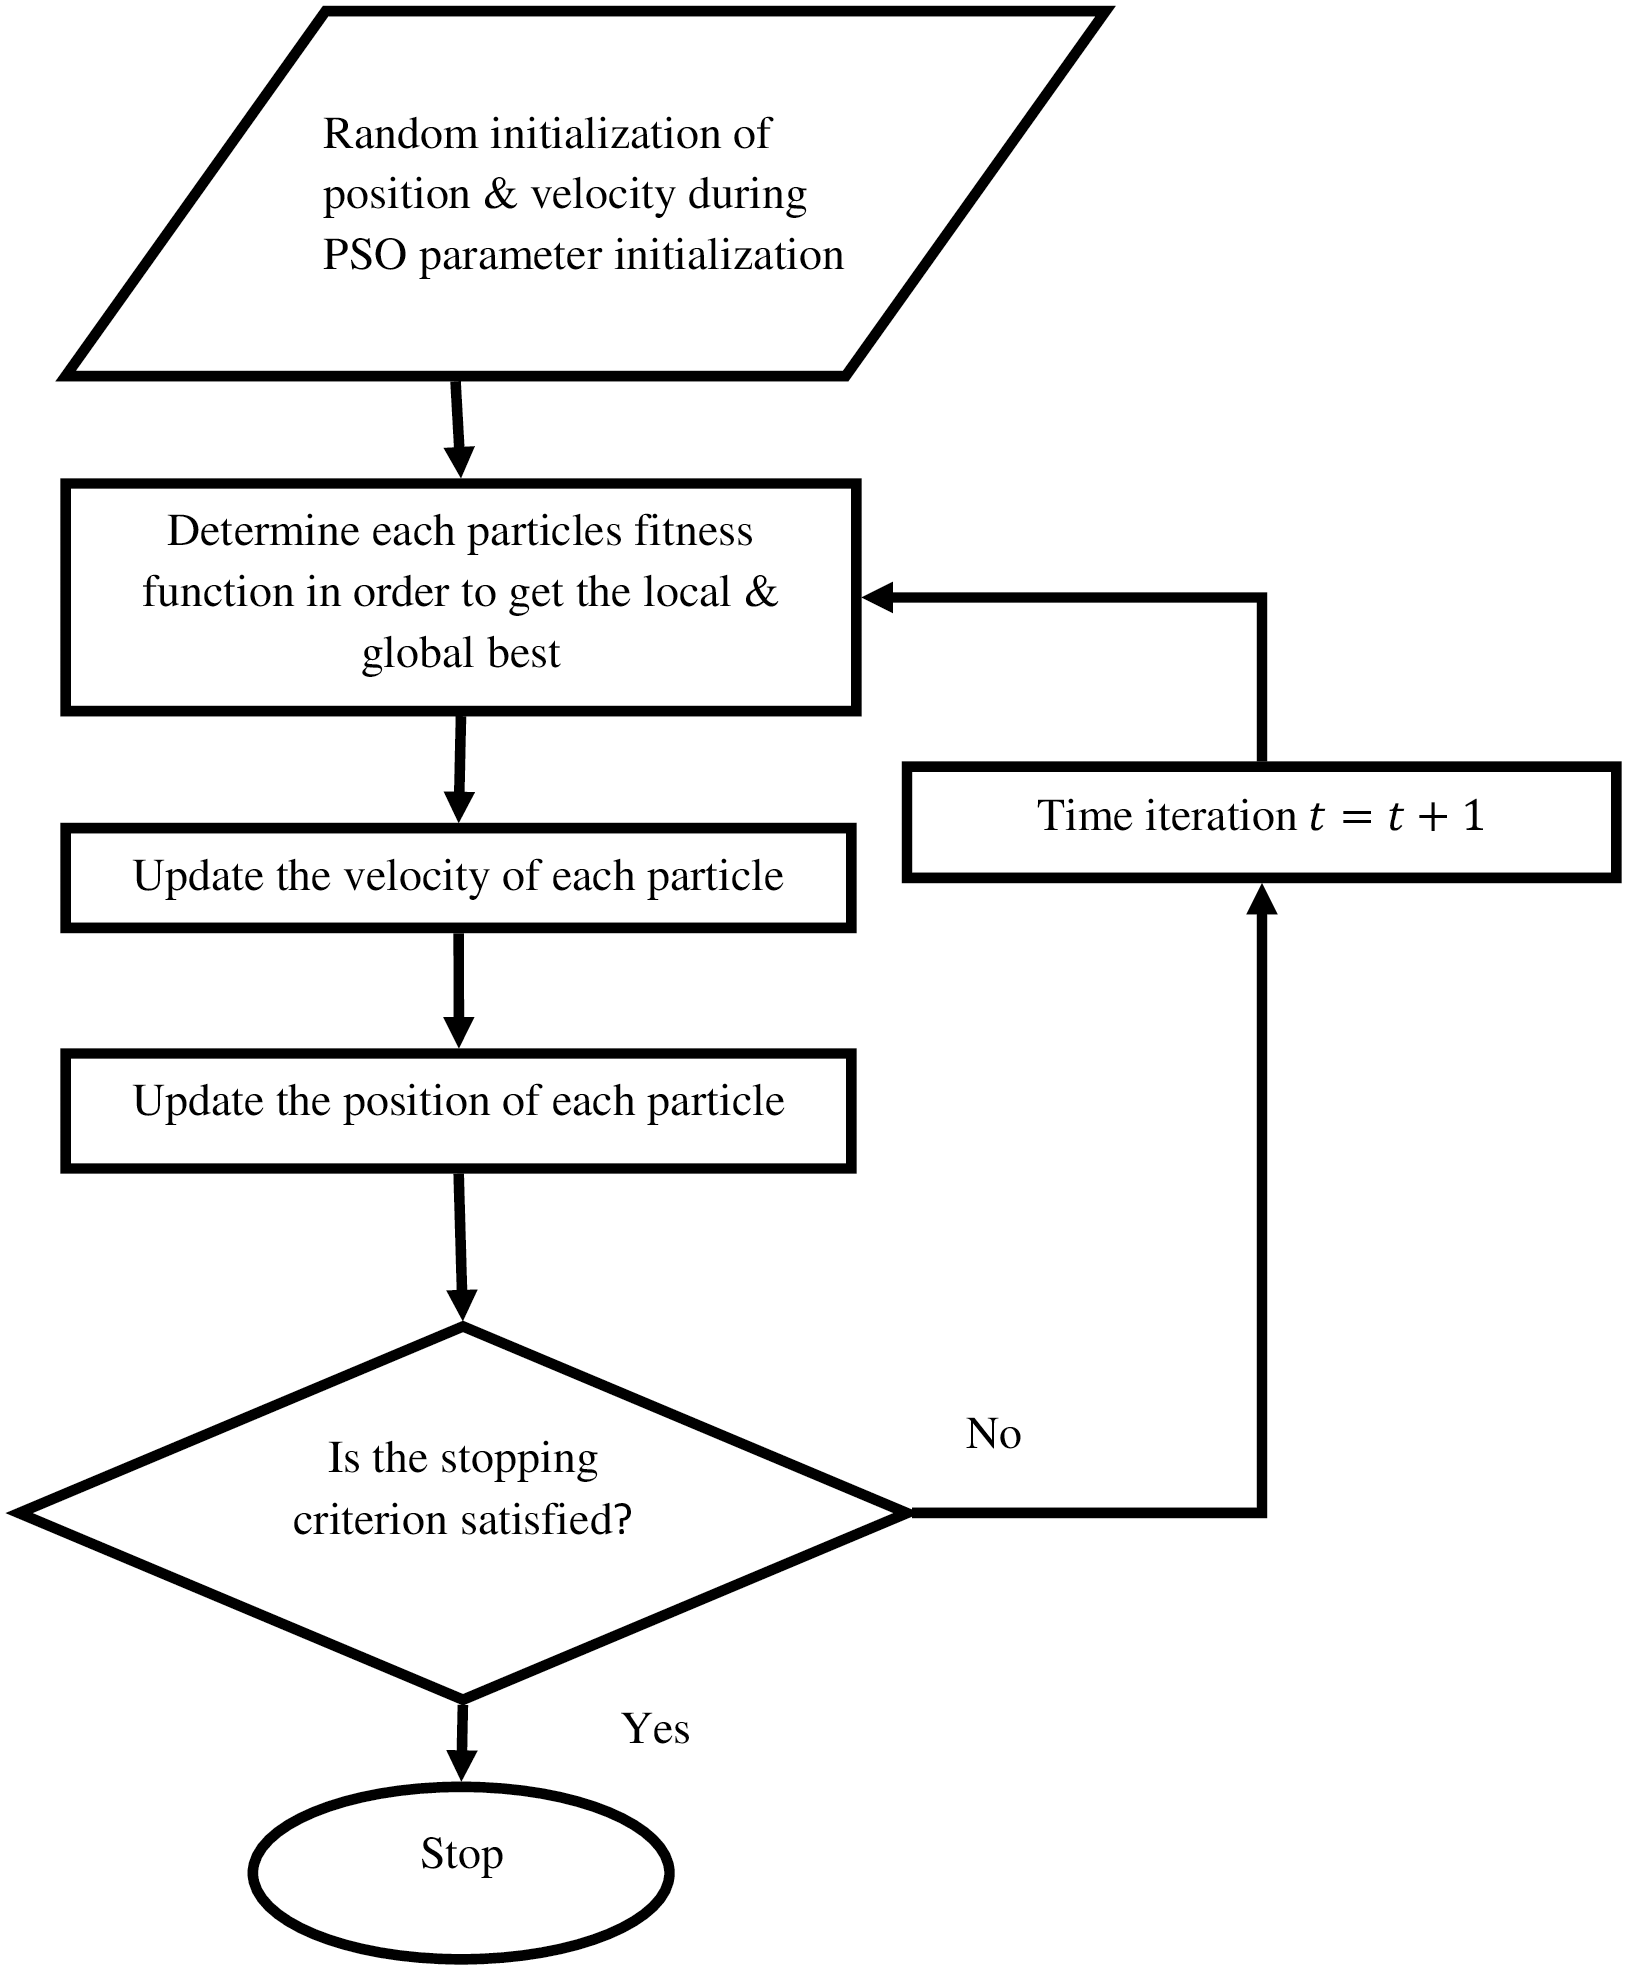
\includegraphics[width=0.5\linewidth]{figures/fig5.Flowchart of PSO algorithm used for tuning quadrotor sliding surface parameters..PNG}

    % Caption for List of Figures (no citation)
    \caption{Flowchart of PSO algorithm used for tuning quadrotor sliding surface parameters} \cite{abera2024improved}

    % Caption shown only under the figure (with citation)
   % \caption*{Source: \cite{abera2024improved}}

    \label{fig:PSO for sliding surface parameters}
\end{figure}

\subsection{Fitness function}


Using the proposed approach, a performance index is used to quantify the optimization 
performance of the quadrotor’s responses. The purpose of the performance index, sometimes 
referred to as the fitness function, is to reduce the differences between the quadrotor’s 
controllable and desired output responses. The goal of this  is to reduce quadcopter 
trajectory tracking error in terms of both position and orientation. Systems constructed 
using Integral Time Absolute Error (ITAE) have minor overshoots and minimal damped 
oscillations. This research utilized the ITAE performance index.

\begin{equation}
ITAE = \int_{0}^{\infty} t |e(t)| \, dt  
\end{equation}


The fittness function used in tunning gains for position controller was as follows:
\begin{equation}
ITAE = \int_{0}^{\infty} t\,\left( |e(x)| + |e(y)| + |e(z)| \right)\, dt
%\tag{4.22}
\label{eq:4.22}
\end{equation}

   The fittness function used in tunning gains for attitude controller was as follows:


\begin{equation}
ITAE = \int_{0}^{\infty} t\,\left( |e(q1)| + |e(q2)| + |e(q3)| \right)\, dt
%\tag{4.23}
\label{eq:4.23}
\end{equation}


Below are the PSO's parameters that were used during tuning for attitude and position controller gains  as shown in Table~\ref{tab:PSO_ITAE_attitude} and Table~\ref{tab:PSO_Position_Gains}.  %


 \small
  \setlength{\arraycolsep}{3pt}  % <-- reduces spacing between columns

  \[
  \mathbf{uba} =
  \left[
  \begin{array}{cccccccccccc}
  100 & 100 & 100 & 100 & 100 & 100 & 100 & 100 & 100 & 100 & 100 & 100
  \end{array}
  \right]
  \]

  \[
  \mathbf{lba} =
  \left[
  \begin{array}{cccccccccccc}
  0 & 0 & 0 & 0 & 0 & 0 & 0 & 0 & 0 & 0 & 0 & 0
  \end{array}
  \right]
  \]

      \[
  \mathbf{ubp} =
  \left[
  \begin{array}{cccccccccccc}
  100 & 100
  \end{array}
  \right]
  \]

  \[
  \mathbf{lbp} =
  \left[
  \begin{array}{cccccccccccc}
  0 & 0 
  \end{array}
  \right]
  \]

  }%
}


  \[
  v_{\max} = 1,\quad
  v_{\min} = 0.1,\quad
  c_{1}=2,\quad
  c_{2}=2
  \]



\[
\textit{Note:}\;
\begin{aligned}
uba      &= \text{upper attitude bound}, \\
lba      &= \text{lower attitude bound}, \\
ubp      &= \text{upper position bound}, \\
lbp     &= \text{lower position bound}, \\
v_{\max} &= \text{maximum particle swarm velocity coefficient}, \\
v_{\min} &= \text{minimum particle swarm velocity coefficient}, \\
c_{1}    &= \text{first particle swarm acceleration coefficient}, \\
c_{2}    &= \text{second particle swarm acceleration coefficient}.
\end{aligned}
\]











\subsection{Adaptive super twisting sliding mode control design}


\textbf{Control structure of adaptive super twisting sliding mode control.} 
After that, super twisting control is considered

\begin{align*}
U_{st} &= -\alpha |\sigma|^{\tfrac{1}{2}} \, \text{sign}(\sigma) + \nu \\[6pt]
\dot{\nu} &= -\tfrac{\beta}{2}\text{sign}(\sigma)
\end{align*}

The adaptive gains are stated as follows:
\begin{align}
\alpha &= \alpha(\sigma, \dot{\sigma}, t) 
\label{4.24} \\[6pt]
\beta &= \beta(\sigma, \dot{\sigma}, t) \label{4.25}
\end{align}

\textbf{Lemma 1.} The adaptation law are to be defined as:

\begin{align}
\dot{\alpha} &=
\begin{cases}
\omega_1 \tfrac{\sqrt{\gamma_1}}{\sqrt{2}} \, \text{sign}(|\sigma|-\mu), & \text{if } \alpha > \alpha_m \\[6pt]
\eta, & \text{if } \alpha \leq \alpha_m
\end{cases} \label{4.26}
\end{align}

\begin{align*}
\beta &= 2 \epsilon \alpha
\end{align*}



The parameters $\epsilon, \gamma_1, \omega, \eta$ are arbitrary positive constants, 
while $\alpha_m$ is a small positive constant.  

\noindent \textbf{Proof.} Lyapunov function candidate is introduced as:
\begin{align}
\nu(\alpha,\beta) = \nu_0 + \tfrac{1}{2\gamma_1}(\alpha-\alpha^*)^2 + \tfrac{1}{2\gamma_2}(\beta-\beta^*)^2 \label{4.27}
\end{align}

where $\nu_0$ is Lyapunov function for $(\sigma,\dot{\sigma})$, 
$\alpha^*, \beta^*$ are maximum possible values of $\alpha, \beta$.



respectively. The derivative of the Lyapunov function is as follows:
\begin{align}
\dot{\nu}(\sigma,\alpha,\beta) &\leq -\eta_0 \sqrt{\nu(\sigma,\alpha,\beta)} 
- |\epsilon_\alpha|\left(\tfrac{1}{\gamma_1}\dot{\alpha} - \tfrac{\omega_1}{\sqrt{2\gamma_1}}\right) \notag \\[6pt]
&\quad - |\epsilon_\beta|\left(\tfrac{1}{\gamma_2}\dot{\beta} - \tfrac{\omega_2}{\sqrt{2\gamma_2}}\right) \label{4.28}
\end{align}

It gives
\begin{align}
\dot{\nu}(\sigma,\alpha,\beta) \leq -\eta_0 \sqrt{\nu(\sigma,\alpha,\beta)} + \zeta \label{4.29}
\end{align}

with
\begin{align}
\zeta &= -|\epsilon_\alpha|\left(\tfrac{1}{\gamma_1}\dot{\alpha} - \tfrac{\omega_1}{\sqrt{2\gamma_1}}\right) 
        - |\epsilon_\beta|\left(\tfrac{1}{\gamma_2}\dot{\beta} - \tfrac{\omega_2}{\sqrt{2\gamma_2}}\right) \label{4.30}
\end{align}

where $\epsilon_\alpha = \alpha - \alpha^*$ and $\epsilon_\beta = \beta - \beta^*$. 
It is evident that the system’s finite-time convergence is assured 
\cite{besnard2007control}.


\begin{table}[htbp]
\centering

\caption[Plant parameter]{Plant parameter.  \cite{bresciani2008modelling}}
\label{tab:Plant parameter for simulation}

\resizebox{\linewidth}{!}{%
\begin{tabular}{|c|c|c|c|}
\hline
\textbf{Plant Parameters} & \textbf{Symbol} & \textbf{Unit} & \textbf{Values} \\ \hline
Thrust coefficient & $b$ & $Ns^2$ & $54.2 \times 10^{-6}$ \\ \hline
Drag factor & $d$ & $Nms^2$ & $1.1 \times 10^{-6}$ \\ \hline
Gravitational Acceleration & $g$ & $m/s^2$ & $9.81$ \\ \hline
The length of the arm of the quadrotor & $\l$ & $m$ & $0.24$ \\ \hline
Mass of quadrotor & $m$ & $Kg$ & $1$ \\ \hline
Inertia around X-axis & $J_{xx}$ & $Nms^2$ & $8.1 \times 10^{-3}$ \\ \hline
Inertia around Y-axis & $J_{yy}$ & $Nms^2$ & $8.1 \times 10^{-3}$ \\ \hline
Inertia around Z-axis & $J_{zz}$ & $Nms^2$ & $14.23 \times 10^{-3}$ \\\hline
%\hline

\end{tabular}
}
\end{table}

Table~\ref{tab:Plant parameter for simulation},  presents different  parameters of quadrotor and Tables~\ref{tab:Design parameter for ASTSMC.}--\ref{tab:Design parameter of adaptation law.}, give the design parameters of the controller,note that values written in Tables ~\ref{tab:Design parameter for ASTSMC.} and \ref{tab:Design parameter for PSO SMC.} were obtained after running a PSO algorithm where as parameters in Table \ref{tab:Design parameter of adaptation law.} were adopted from article \cite{abera2024improved}.  

\textbf{Remark 1.}  In order to achieve best trajectory tracking optimal gain was  obtained using PSO technique.

%Simulation results for optimal STSMC that is adaptive are presented here in where as mathematical model used captures some of the dynamics ignored in most of currennt literatures.


\begin{table}[h!]
\centering
\caption{Design parameter for PSO SMC.}
\begin{tabular}{|l|c|}
\hline
\textbf{Parameter} & \textbf{Value} \\ \hline
$\lambda_x,$\lambda_y,$\lambda_z, & 80,80,80 \\ \hline

 $ \lambda_{q_1},  \lambda_{q_2}$   \lambda_{q_3}& 100,83.4608,100 \\ \hline
$c_z, c_z, c_z$ & 1,1,1 \\ \hline
$ c_{q_1}, c_{q_2}, c_{q_3}$ & 0.2351,68.7297,32.0515 \\ \hline

\end{tabular}
\label{tab:Design parameter for PSO SMC.}
\end{table}




\begin{table}[h!]
\centering
\begin{minipage}{0.48\linewidth}
\centering
\caption{Design parameters for ASTSMC}
\label{tab:astsmc_params}
\begin{tabular}{|l|c|}
\hline
\textbf{Parameter} & \textbf{Value} \\ \hline
$a_x,a_y,a_z$ & 0.01, 0.01, 0.01 \\ \hline
$a_{q1},a_{q2},a_{q3}$ & 43.4506, 34.2058, 51.4594 \\ \hline
$\beta_x,\beta_y,\beta_z$ & 0.0002, 0.0002, 0.0002 \\ \hline
$\beta_{q1},\beta_{q2},\beta_{q3}$ & 100, 0, 0.0426 \\ \hline
\end{tabular}
\label{tab:Design parameter for ASTSMC.}
\end{minipage}
\hfill
\begin{minipage}{0.48\linewidth}
\centering
\caption{Design parameters of adaptation law}
\label{tab:adapt_params}
\begin{tabular}{|l|c|}
\hline
\textbf{Parameter} & \textbf{Value} \\ \hline
$\omega_1$ & 0.0001 \\ \hline
$a_m$ & 0.01 \\ \hline
$\eta$ & 0.01 \\ \hline
$\gamma_1$ & 2 \\ \hline
$\mu$ & 0.7 \\ \hline
\end{tabular}
\label{tab:Design parameter of adaptation law.}
\end{minipage}
\end{table}

\section{Experimental Validation}

\begin{table}[h]
\centering
\caption{Hardware components used in the quadrotor system}
\label{tab:hardware}
\begin{tabular}{|c|l|l|}
\hline
S/No & Item & Specs \\ 
\hline
01 & Teensy & 4.0 \\ 
02 & MPU6050 & GY-521 \\ 
03 & Spacer & M3 $\times$ 25mm \\ 
04 & Battery & 3S / 11.1V 460mAh \\ 
05 & Emax ESC & BLHeli-12A \\ 
06 & Brushless motor & ECO 1106-4500KV \\ 
07 & Battery Connector & XT60 \\ 
08 & RC transmitter & FS-I6X \\ 
09 & Receiver FS-IA6B & PWM 6CH 2.4GHz \\ 
10 & Power switch & BTS50055-1TMB \\ 
11 & Resistor & 100$\Omega$, 510$\Omega$, 2000$\Omega$ \\ 
12 & Zener Diode & BZX55C2V4 \\ 
13 & Female to Female Jumper wires & -- \\ 
14 & LEDs & Red and Green -- 5V \\ 
15 & Lower and Upper frame & CarbonAeronautics \\ 
16 & USB & A to Micro B \\ 
17 & Slide switch & OS102011MS2QN1C \\ 
18 & Gemfam propeller & 2218 3-blades \\ 
\hline
\end{tabular}
\end{table}

\subsection*{A. Hardware Architecture}

The hardware architecture of the custom quadcopter platform was composed of a modular embedded control system, sensing units, power electronics, propulsion components, and a lightweight mechanical structure as shown in ``Table\ref{tab:hardware}. The Teensy 4.0 microcontroller was used as the main flight controller and executed the attitude control algorithms while handling communication with onboard sensors, actuators, and the radio receiver. It was mounted at the center of the airframe using M3 $\times$ 25 mm spacers to provide mechanical stability and reduce vibration transmission.

Attitude sensing was achieved using an GY-521 MPU6050 inertial measurement unit, which provided angular rate and acceleration measurements. The IMU was interfaced with the Teensy via the I$^2$C communication bus and was positioned close to the quadcopter’s center of mass to improve measurement accuracy. Signal conditioning and voltage protection were implemented using resistors (100~$\Omega$, 510~$\Omega$, and 2~k$\Omega$) and a BZX55C2V4 Zener diode to ensure reliable operation of the embedded electronics.

The propulsion system consisted of four ECO 1106--4500 KV brushless DC motors, each driven by an EMAX BLHeli-12A electronic speed controller (ESC). The ESCs received pulse-width modulation (PWM) control signals from the Teensy and regulated the motor speeds accordingly. Gemfan 2218 three-blade propellers were mounted on the motors to generate the thrust and control torques required for quadcopter stabilization and maneuvering.

Electrical power was supplied by a 3S (11.1~V), 460~mAh LiPo battery, which was connected through an XT60 battery connector to support the high current demands of the propulsion system. A BTS50055-1TMB power switch and a slide switch (OS102011MS2QN1C) were integrated into the power distribution line to enable safe and controlled power management. System status indications, including power availability and alarming state, were provided using 5~V red and green LEDs.

Pilot commands were transmitted using an FS-I6X radio transmitter and received by an FS-IA6B 6-channel PWM receiver, which was directly interfaced with the Teensy input pins. This configuration allowed real-time manual command input while maintaining compatibility with onboard control algorithms. Female-to-female jumper wires were used for signal routing between components during assembly and testing.

The mechanical structure was formed using upper and lower Carbon Aeronautics frames. which provided a rigid and lightweight airframe suitable for experimental flight tests. 
A USB Type-A to Micro-B cable was used for firmware upload, debugging, and data logging during ground-based experiments. 
The complete assembly is shown in Fig.\ref{fig:quadcopter_setup}.

%\begin{figure}
   % \centering
   % 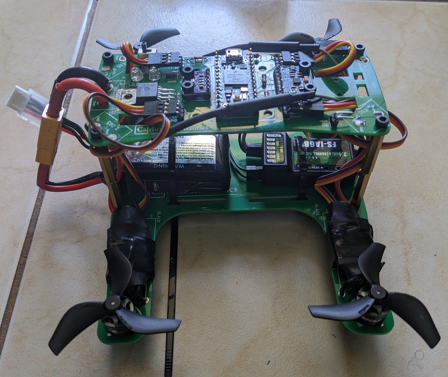
\includegraphics[width=1\linewidth]{figures/assembled Quadcopter.png}
    %\caption{Custom  Assembled Quadcopter}
   % \label{fig:Custom  Assembled Quadcopter}
%\end{figure}

%\begin{figure}
  %  \centering
   % 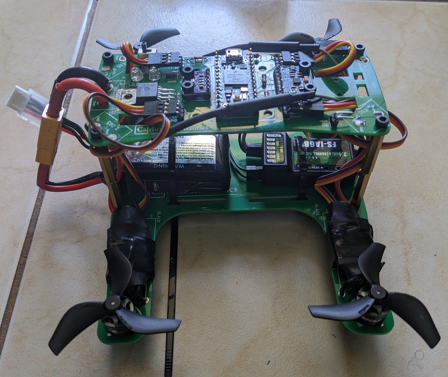
\includegraphics[width=1\linewidth]{figures/assembled Quadcopter.png}
   % \caption{Assembled Quadcopter Mounted on custom UAV test rig ready for experiments.}
   % \label{fig: Assembled Quadcopter on testrig}
%\end{figure}


%%%%%%%%%%%%%%%%%
\begin{figure}[htbp]
    \centering
    
    \begin{subfigure}{0.48\textwidth}
        \centering
        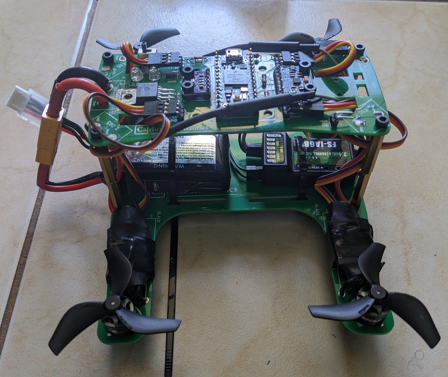
\includegraphics[width=\linewidth]{figures/assembled Quadcopter.png}
        \caption{Custom assembled quadcopter}
        \label{fig:assembled_quadcopter}
    \end{subfigure}
    \hfill
    \begin{subfigure}{0.48\textwidth}
        \centering
        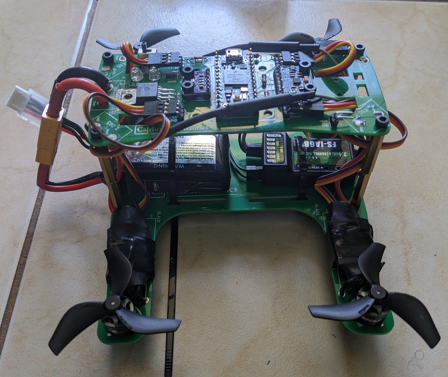
\includegraphics[width=\linewidth]{figures/assembled Quadcopter.png}
        \caption{Quadcopter mounted on custom UAV test rig}
        \label{fig:quadcopter_testrig}
    \end{subfigure}
    
    \caption{Experimental quadcopter platform and test setup}
    \label{fig:quadcopter_setup}
\end{figure}



\subsection*{B.	Sensor Processing}
Sensor processing was implemented to obtain reliable attitude-related measurements required for real-time control of the custom quadcopter. The primary sensing unit used in the platform was the MPU6050 6-DOF inertial measurement unit, which provided three-axis angular velocity and three-axis linear acceleration data. These measurements were used to estimate the quadcopter's attitude and angular rates during flight.

Gyroscope data were sampled at a fixed rate synchronized with the control loop execution. Prior to flight, a gyroscope calibration procedure was performed while the quadcopter was kept stationary. During this process, multiple samples were collected and averaged to estimate constant bias offsets for each axis. These offsets were then subtracted from subsequent gyroscope measurements to reduce steady-state drift.

To mitigate the effects of high-frequency noise caused by motor vibrations and structural resonances, the raw gyroscope signals were processed using a digital low-pass filter. This filtering step improved measurement smoothness while preserving the dynamic response required for attitude control. Accelerometer data were also filtered and normalized to provide a reference for gravity direction, which was essential for correcting long-term drift in orientation estimation.

Attitude estimation was achieved by combining gyroscope and accelerometer measurements using a lightweight sensor fusion algorithm suitable for real-time embedded implementation. The algorithm updated the orientation representation at each control cycle and provided roll, pitch, and yaw information required for feedback control. The chosen approach was computationally efficient and compatible with the limited latency requirements of the embedded system.

All sensor processing operations were executed onboard the Teensy 4.0 microcontroller using floating-point arithmetic. The processed angular rates and attitude estimates were made available to the control algorithm at each control step, ensuring consistent and time-aligned feedback. This sensor processing framework provided accurate and robust attitude information, enabling stable flight and reliable experimental validation of the proposed control strategy.

\subsection*{C.Control Law}

The attitude control of the quadcopter was achieved using an Adaptive Super-Twisting Sliding Mode Controller (ASTSMC). The controller was designed to regulate the quadcopter's rotational dynamics about the roll, pitch, and yaw axes in the presence of model uncertainties, external disturbances, and actuator nonlinearities. This approach was selected to overcome the limitations of conventional PID controllers, particularly their sensitivity to disturbances and parameter variations.

The control design was formulated in the angular-rate domain. For each rotational axis, a sliding surface was defined using a combination of the tracking error and its derivative. The sliding surface represented the desired dynamic behavior of the closed-loop system and served as the basis for control action generation. By enforcing convergence of the sliding surfaces to zero, accurate attitude stabilization was achieved.

To reduce the chattering effect commonly associated with first-order sliding mode control, the super-twisting algorithm was employed. This higher-order sliding mode technique generated a continuous control signal while ensuring finite-time convergence of the sliding variables. As a result, smooth actuator commands were obtained without sacrificing robustness.

An adaptive mechanism was incorporated into the control law to update the sliding surface gains online. These gains were adjusted based on the magnitude of the sliding variables, allowing the controller to automatically increase robustness under high disturbances and reduce control effort during steady-state operation. This adaptive feature improved tracking performance and enhanced stability across different flight conditions.

The control law was implemented in discrete time and executed at a fixed sampling period on the Teensy 4.0 microcontroller. The controller outputs were mapped to pulse-width modulation (PWM) signals, which were sent to the electronic speed controllers to regulate motor speeds. Control saturation limits were applied to ensure safe operation within actuator constraints.

\subsection*{Embedded Implementation}

The controller was implemented in C++ using the Arduino Teensyduino environment. Floating-point arithmetic and interrupt-driven timing ensured deterministic execution.


\clearpage


